\documentclass[11pt,a4paper]{article}
\usepackage[margin=2.4cm]{geometry}
\usepackage[T1]{fontenc}
\usepackage{booktabs}
\usepackage{array}
\usepackage{xcolor}
\usepackage{titlesec}
\usepackage{enumitem}
\usepackage{tcolorbox}
\usepackage{graphicx}
\usepackage{amsmath}
\usepackage{amssymb}
\usepackage{longtable}
\usepackage[hidelinks]{hyperref}

\definecolor{good}{HTML}{1B7F3B}
\definecolor{warn}{HTML}{B26B00}
\definecolor{bad}{HTML}{B3261E}
\definecolor{grey}{HTML}{666666}
\definecolor{rule}{HTML}{2B4C7E}

\newcommand{\code}[1]{\texttt{#1}}
\newcommand{\dn}{\textcolor{good}{\textbf{done}}}
\newcommand{\fl}{\textcolor{warn}{\textbf{in flight}}}
\newcommand{\ns}{\textcolor{grey}{not started}}
\newcommand{\done}{\textcolor{good}{\textbf{DONE}}}
\newcommand{\prog}{\textcolor{warn}{\textbf{IN PROGRESS}}}
\newcommand{\todo}{\textcolor{grey}{\textbf{NOT STARTED}}}
\newcommand{\solid}{\textcolor{good}{\textbf{solid}}}
\newcommand{\weak}{\textcolor{warn}{\textbf{weak}}}
\newcommand{\unsup}{\textcolor{bad}{\textbf{unsupported}}}

% the five outcomes a mechanism can have against the promoted language (see the contract box, S2)
\newcommand{\cNew}{\textcolor{good}{\textbf{new word}}}
\newcommand{\cImpl}{\textcolor{rule}{\textbf{another way}}}
\newcommand{\cAlias}{\textcolor{grey}{\textbf{already had it}}}
\newcommand{\cRef}{\textcolor{warn}{\textbf{widen a word}}}
\newcommand{\cOut}{\textcolor{grey}{no biology}}
\newcommand{\cUnk}{\textcolor{bad}{\textbf{unclassified}}}

\titleformat{\section}{\large\bfseries\color{rule}}{\thesection.}{0.6em}{}
\titleformat{\subsection}{\normalsize\bfseries}{}{0em}{}
\setlist[itemize]{leftmargin=1.1em,itemsep=2pt,topsep=3pt}
\setlength{\parskip}{5pt}
\setlength{\parindent}{0pt}
\renewcommand{\arraystretch}{1.25}

\newtcolorbox{phasebox}[1]{colback=white,colframe=rule!55,boxrule=0.7pt,
  arc=2pt,left=8pt,right=8pt,top=6pt,bottom=6pt,title={\bfseries #1},
  fonttitle=\color{white},colbacktitle=rule}

\title{\textbf{Plexus Atlas --- jax-morph}\\[6pt]
\large Progress note --- written to be read, not decoded}
\author{}
\date{31 July 2026}

\begin{document}
\maketitle
\vspace{-2.2\baselineskip}

\begin{center}\small\color{grey}
The twin of \texttt{plexus2\_discovery.pdf}, for the other half of the programme.\\
Plain English throughout. Organised by phase, because phases are where we stop and you decide.
\end{center}

\vspace{4pt}
\hrule
\vspace{10pt}

%======================================================================
\section{What we are doing --- the second way to grow the language}

There are two ways to grow the Plexus vocabulary, and as of today both are running.

\textbf{Discovery} (the Okuda folder) searches for a mechanism nobody has written down. It
proposes a change to the model's structure, says what it expects \emph{before} running, runs, and
records whether it was right. It is the harder science and the slower loop.

\textbf{Atlas} (this folder) is the other one, and it is what Appendix~E of the Plexus~2 paper
promises. It takes a published system whose code \emph{exists}, reads that code, and asks a
narrower question: \emph{can the Plexus operator algebra say everything this framework says?}
Whatever the language cannot say becomes a new operator. Whatever it can say twice over is
evidence that the language is converging on something real.

\textbf{The target is jax-morph} --- Deshpande, Mottes \emph{et al.}, \emph{Engineering
morphogenesis of cell clusters with differentiable programming} (Nature Computational Science,
2025). Cells as soft particles that grow, divide, die, push on one another, secrete and read
chemical signals, and decide what to do next through a small gene network. Apache licensed, pure
Python, 24 mechanisms --- and, the point, it runs.

\textbf{Two deliverables, and neither one alone is enough.}

\begin{enumerate}
\item \textbf{The figure.} One headline result of the paper, reproduced inside Plexus out of
operators translated from their code --- not fitted to their output.
\item \textbf{The ledger.} Every mechanism in the repository sorted into one of three buckets:
something the promoted language already has, something it has but must widen, or something
genuinely new.
\end{enumerate}

The figure without the ledger is a demo. The ledger without the figure is a spreadsheet nobody
has checked against reality.

\begin{tcolorbox}[colback=grey!6,colframe=grey!45,boxrule=0.7pt,arc=2pt]
\textbf{What we compare against: the promoted language, and nothing else.} 52 registered operator
contracts in \code{plexus.operators} --- validated, importable, typed, in the engine. Code sitting
in \code{prototype/} or in the \code{candidates/} anti-chamber is not part of the language and
does not enter this measurement. Measuring against code nobody has reviewed would be measuring
the wrong thing.
\end{tcolorbox}

%======================================================================
\section{What a contract is --- the unit everything else is counted in}\label{sec:contract}

Every number in this note is a count of \emph{contracts}, so the word has to mean something
precise before any of them can be read.

\begin{tcolorbox}[colback=rule!4,colframe=rule!55,boxrule=0.9pt,arc=2pt]
\textbf{A contract is the typed signature of a verb --- not a piece of code.} It is fixed by five
things and nothing else:

\begin{enumerate}[leftmargin=1.5em,itemsep=1pt]
\item its \textbf{name} --- the verb: \code{divide}, \code{adhere}, \code{regulate};
\item the \textbf{set} it acts on (cells, a grid, a graph of contacts);
\item the state fields it \textbf{reads};
\item the state fields it \textbf{writes};
\item its \textbf{kind} --- whether it overwrites a field to a constraint, contributes a rate to
be integrated, or fires as a discrete event; and whether it crosses a \textbf{map} between sets.
\end{enumerate}

\textbf{Two mechanisms hold the same contract when a spec could swap one for the other and change
nothing else.} Same set, same reads, same writes, same kind. They may compute utterly different
arithmetic in between --- that is not what a contract is about.
\end{tcolorbox}

That definition is doing real work, and it is worth seeing where. jax-morph computes the change in
a cell's gene state in four different places: through a dense matrix, through a neural network,
through a thermodynamic binding law, and in a base class that integrates whichever one it is
handed. Four files, four papers' worth of modelling tradition, four sets of parameters. All four
read \code{gene} and a sensed drive, all four write \code{gene}, all four emit a rate integrated
over one macro-step. \textbf{That is one word --- \code{regulate} --- spoken four ways.}

Counting them as four new contracts would have inflated the headline number by 36\% on the single
measurement this whole apparatus exists to make. So the ledger counts \textbf{distinct contracts},
and every mechanism lands in exactly one of five outcomes:

\begin{center}
\small
\begin{tabular}{@{}l p{11.9cm}@{}}
\toprule
\cAlias & the promoted language already has this word, registered and validated.\\
\cRef & it has the word, but the registered signature must \emph{widen} to admit this. The record
forces the cost of widening to be written down.\\
\cNew & the promoted language has no word for this. This is the only outcome that moves the
curve.\\
\cImpl & a second mechanism reaching a contract this run has already counted as new. A different
numerical realisation of the same verb --- \emph{not} new vocabulary.\\
\cOut & no biology to extract: the framework's own infrastructure, or a null default.\\
\bottomrule
\end{tabular}
\end{center}

\textbf{And the record does not get the last word on its own verdict.} Each entry carries the
verdict its normalizer argued for, one mechanism at a time. The ledger recomputes across the whole
run --- it can see what the normalizer could not, namely that some earlier entry already claimed
this contract --- and where the two disagree, \textbf{the ledger wins and the disagreement is
printed}. Today fourteen entries argue \emph{new}; eight contracts are new. Six of those fourteen
are the same six words said twice, and the ledger says so by name.

That is the difference between counting words and counting files, and it is the only reason the
saturation curve means anything.

%======================================================================
\section{Where we actually are}

\textbf{Phases 0 to 3 are done.} Every one of the 24 mechanisms has been read at source,
normalized into a typed Plexus contract, attacked by a skeptic, and --- where it was new or a
refinement --- implemented as a Plexus operator with a test. Sixteen operator modules exist,
\textbf{all sixteen import, register the implementation their record claims, agree with their
recorded signature, pass a test, and co-exist in one registry}.

\textbf{The first ledger is in.} Eight genuinely new contracts, six further implementations of
them, two aliases of things we already had, two refinements, six entries with no biology to
extract. And the forward composition RUNS: the authors' proliferation model, rebuilt from those
operators, grows a jammed cluster from 4 cells to 124 --- against their 82. That last disagreement
is the most useful number the atlas has produced, and \S\ref{sec:fwd} is about it.

\begin{center}

\includegraphics[width=0.62\textwidth]{_state/saturation.png}\\
{\small\color{grey}The measurement, as far as it goes. The dotted line is the world in which every
mechanism is new vocabulary; the steps are what actually happened. One repository cannot show
saturation --- the second and third can.}
\end{center}

%======================================================================
\section{Did we reproduce the paper? --- the short answer}\label{sec:short}

Three questions deserve answering before any of the machinery below, in plain English.

\begin{tcolorbox}[colback=grey!6,colframe=grey!45,boxrule=0.8pt,arc=2pt]
\textbf{Did we reproduce it?} \emph{Partly, and the part we did is the harder one to fake.} Their
\textbf{forward model} --- the proliferating cell cluster their library ships as its worked
example --- runs inside Plexus out of operators translated from their code, and every one of its
mechanisms has been checked against their own running implementation. Their \textbf{Figure 5} ---
engineered morphogenesis, where a gene network is \emph{optimised} until the cluster
self-organises into a specified shape --- is \textbf{not} reproduced yet. That is Phase 6, and it
is in progress.
\end{tcolorbox}

\textbf{What is the same.}

\begin{itemize}
\item \textbf{Every mechanism, to a number.} Sixteen differential tests against the authors' code
running in its own interpreter, each with its metric and threshold written down \emph{before} the
run. Disagreements from $2{\cdot}10^{-16}$ to $1{\cdot}10^{-2}$, every one under a bar argued from
numerics rather than chosen to fit.
\item \textbf{The morphology.} Both engines jam into a round, confluent cluster of uniformly-sized
cells (\S\ref{sec:fwd}).
\item \textbf{The size.} Radius of gyration $0.651 \to 3.228$ against $0.686 \to 3.518$ --- 9\%
over the whole run, on the observable that is robust to the random seed.
\item \textbf{The division mechanism.} Pooled division hazard agrees to $1.1{\cdot}10^{-3}$
against a three-sigma bar of $5.2{\cdot}10^{-3}$, over 48 seeds and $\sim$47{,}000 cell-steps a
side.
\item \textbf{The architecture, unexpectedly.} jax-morph is itself built from composable physics
steps that declare which state they read and write and compose by operator splitting. Two groups
arrived at nearly the same decomposition from opposite directions.
\end{itemize}

\textbf{What is different.}

\begin{itemize}
\item \textbf{The cell count: 82 against 124.} Two engines drawing from independent random streams
produce different realisations of the same process, so this compares luck, not mechanism --- which
is why the differ refused to compare counts at all and compared the hazard instead. It is the
figure's subject, not its failure.
\item \textbf{Four places where their code contradicts their paper}, and we follow the code. Their
growth law is a saturating von Bertalanffy flow, not the paper's constant increment with a
\code{min} clamp. Their gene network mixes the sensed input \emph{inside} the sigmoid through a
trainable matrix, not added outside it. Their Morse potential carries a smooth cutoff the paper's
equation does not have. Their stress is an Irving--Kirkwood virial, not the paper's taxicab sum.
\textbf{Recording those contradictions is among the most valuable things this reproduction
produced}, and none of them is visible without the code.
\item \textbf{Two mechanisms exist in the code and nowhere in the paper}: cell death, and
self-propelled (active Brownian) motion. The library ships capability the publication does not
claim.
\item \textbf{One operator is deliberately less capable than theirs.} Their mechanical relaxation
differentiates the \emph{equilibrium} by the implicit function theorem; ours equilibrates
faithfully but forward-only, and says so (\code{DIFFERENTIABLE = False}).
\item \textbf{And Figure 5 itself}, which is the honest headline of this list.
\end{itemize}

\textbf{What it cost the language} --- the measurement the atlas exists to make --- is eight
genuinely new contracts out of 24 mechanisms, with six further implementations of those same
eight, two aliases, two refinements, and six entries that model no biology at all. A yield of 0.44
new contracts per scored mechanism, on the first repository.

%======================================================================
\section{Why a target with code changes everything}

\begin{tcolorbox}[colback=rule!4,colframe=rule!55,boxrule=0.7pt,arc=2pt]
\textbf{The thing Okuda could never give us: an answer to compare against.}

Okuda \emph{et al.} published a paper with no code. So when our tube looks wrong there are three
explanations and no way to separate them: the operator is wrong, the parameter is wrong, or we
read the figure wrong. Days of the discovery campaign went into exactly that fog.

Here the authors' own implementation sits in \code{papers/jax-morph} and, as of today, \emph{runs}
on this machine in its own isolated Python. We can put our reconstruction and their implementation
on the same initial condition and subtract. Faithfulness stops being a judgement and becomes a
number, against a threshold written down in advance.
\end{tcolorbox}

There is a second reason, and it is the more interesting one. jax-morph is not merely a simulator:
it is built from \emph{composable physics steps} that compose by operator splitting, declare which
state fields they read and write, and are cross-validated when a model is assembled. That is,
independently, most of the Plexus thesis. If two groups arrived at nearly the same decomposition
from opposite directions, the decomposition is probably not arbitrary --- and the places where
they differ are where we should expect to learn something.

Three differences are already visible from their documentation, before any agent has read a line:

\begin{itemize}
\item They classify a step by its \textbf{time-scale}: a fast constraint solved at the current
configuration, a finite-rate process, or an instantaneous event. Plexus classifies an operator by
\emph{which part of the state it touches}. The two are orthogonal, and we do not have theirs.
\item Their randomness has a \textbf{contract}: a stochastic step records what it sampled, can
replay it, and can score it --- which is what makes a discrete event like cell division
differentiable at all. Plexus has no such contract.
\item Their macro-step is an \textbf{explicit first-order operator split} with a stated error
term. Ours is a schedule.
\end{itemize}

None of those three is a biological operator. All three are candidates to improve the
\emph{language}, which is the second thing the atlas is for.

%======================================================================
\section{What is genuinely working}

Everything here was run today, and its output checked.

\begin{center}
\small
\begin{tabular}{@{}p{4.3cm} l p{8.7cm}@{}}
\toprule
\textbf{piece} & \textbf{state} & \textbf{what was verified}\\
\midrule
frozen baseline & \dn &
52 registered contracts, 42 canonical and 10 aliases, across 10 families. Written to a file, so
the measurement cannot drift while it is being taken.\\

the oracle & \dn &
jax-morph 0.4.0 installed from our local clone (\code{ace08b8}) into its own interpreter. Nothing
in the Plexus environment can import it.\\

oracle determinism & \dn &
the authors' proliferation model, run twice from one seed, is \emph{bit-identical}. Without this,
a later disagreement could be their noise rather than our error.\\

first reference run & \dn &
4 cells $\to$ 82 over 40 macro-steps; cluster radius 0.65 $\to$ 3.23; the division buffer never
overflows. Trajectory, summary and figure on disk, each with its provenance.\\

record + validator & \dn &
twelve rules. Self-tested against a record built to break every one: all twelve fire, and a
well-formed record passes in silence.\\

saturation ledger & \dn &
self-tested, including its right to overrule the record: a ``new'' whose name is already
registered is demoted to \emph{alias} and the disagreement is reported, not applied quietly.\\

mechanism inventory & \dn &
24 mechanisms from the clone's syntax tree --- 20 classes plus 4 architectural contracts that are
not classes and that a scan alone would have missed.\\

the guarded driver & \dn &
every agent call is a transaction: blast radius, rung, twelve rules, then commit or revert.\\

one live agent call & \dn &
excavator on \code{Division}: committed in 6.3 minutes, nine reimplementer traps, verdict
correctly left blank, and an explicit list of what it could \emph{not} establish.\\

the paper, readable & \dn &
29 pages, 14{,}142 words, extracted with page markers and greppable --- because the first agent
call discovered it could not open the PDF.\\
\bottomrule
\end{tabular}
\end{center}

\begin{center}

\includegraphics[width=\textwidth]{_oracle/runs/smoke/reference.png}\\
{\small\color{grey}The reference, running here. Their model, their code, our machine: mechanical
relaxation under a Morse potential, saturating growth, stochastic division. All six panels share
one spatial scale --- the discovery loop spent a day being fooled by panels that did not.}
\end{center}

%======================================================================
\section{The team of agents --- what is switched on}

Six roles, each seeing one mechanism at a time.

\begin{center}
\small
\begin{tabular}{@{}l p{7.9cm} l l@{}}
\toprule
\textbf{role} & \textbf{what it does} & \textbf{may edit} & \textbf{budget}\\
\midrule
excavator & reads the mechanism at source: what it does to the state, the equations, the role of
every knob, and what a reimplementer would get wrong. Forbidden from judging novelty. & the record
& 10 min\\
normalizer & writes it as a typed Plexus operator and commits to a verdict, with the whole
promoted language in front of it. & the record & 8 min\\
skeptic & tries to \emph{refute} that verdict, in whichever direction it went; defaults to refuted
when unsure. & \textbf{nothing} & 5 min\\
implementer & writes the Plexus operator into the anti-chamber, with a test of one property
statable without the reference. & code & 15 min\\
differ & writes one metric and one threshold \emph{first}, then runs both implementations on the
same initial condition. & code + record & 12 min\\
curator & promotes, or refuses to. Refusal is a result. & code + docs & 10 min\\
\bottomrule
\end{tabular}
\end{center}

\subsection{The agents have no authority over the record}

This is the part I would ask you to check hardest, because it is the lesson from the other folder.
Every discovery-loop error came from a measurement nobody had checked, written down by an agent
doing its best. So here the agents decide nothing. They edit; the driver decides whether the edit
survives.

\begin{enumerate}[leftmargin=1.4em]
\item \textbf{Blast radius.} Only the mechanism it was given may have changed. An agent that tidies
a neighbouring entry in passing has destroyed our ability to attribute anything, so the whole call
is thrown away.
\item \textbf{Rung.} Each role can only reach its own status. The excavator cannot declare
something validated. A rung is earned by an artefact --- a code path that resolves, a module that
imports, an oracle run on disk --- never by an assertion.
\item \textbf{The twelve rules.} If the record does not validate, the edit is reverted and the
violations are handed back to the agent, \emph{once}. A second failure marks the mechanism
\textbf{blocked} and leaves it for a human. It is never silently skipped.
\end{enumerate}

Every revert is logged with the agent's own words, so a systematic misunderstanding shows up as a
pattern rather than as noise. A call that changes \emph{nothing} also counts as a failure: the
record is the product, and an agent that explains a brilliant normalization in prose has produced
nothing.

\subsection{The four ways this measurement could still lie}

\begin{center}
\small
\begin{tabular}{@{}p{3.4cm} p{11.6cm}@{}}
\toprule
\textbf{failure} & \textbf{what stops it}\\
\midrule
inflated novelty & the ledger re-derives every ``new'' against the frozen baseline itself and
reports disagreement with the record by name.\\
flattering aliases & calling two things the same operator hides a lost capability. The skeptic is
aimed at this specifically, and a refinement must state what it breaks for existing users.\\
a threshold chosen after the fact & the differ writes metric and threshold into the record before
running anything. A criterion no valid configuration could meet is exactly how the discovery loop
lost a week.\\
a contaminated oracle & the reference lives in a separate interpreter. A Plexus process that could
import it could borrow its answer, and a test that can be contaminated is not a test.\\
\bottomrule
\end{tabular}
\end{center}

%======================================================================
\section{The phases}

Seven stages. \textbf{I stop at the end of each one and wait for you.} That is the partition.

\begin{phasebox}{Phase 0 --- Instruments and the frozen baseline \hfill \done\ (16 of 16)}
\textbf{Goal.} Make every later measurement trustworthy \emph{before} taking one. Nothing here is
science; each item makes a question askable.

\textbf{What had to be done}
\begin{enumerate}[leftmargin=1.5em,itemsep=1pt]
\item Choose a target with running code, a licence we can build on, and biology worth having.
\item Freeze what Plexus can already say, before reading a line of the target.
\item Put the reference in its own interpreter, and forbid it in ours.
\item Prove the reference is deterministic at a fixed seed.
\item Produce the first reference artefact, and check it against its own figure.
\item Make every reference artefact carry the code and the versions that made it.
\item Refuse a reference run that hits an array bound instead of a biological limit.
\item Write the record down as \emph{rules}, not as a template.
\item Self-test the rules against a record built to break every one of them.
\item Let the ledger overrule the record, and report the disagreement.
\item Self-test that overruling.
\item Extract the mechanism inventory mechanically, not from memory.
\item Add the mechanisms that are not classes and that a scan cannot see.
\item Make every agent call a guarded transaction.
\item Run one real agent call end to end before trusting the plumbing.
\item Make the paper itself readable to an agent.
\end{enumerate}
\end{phasebox}

\begin{phasebox}{Phase 0 --- what actually happened, point for point}
\footnotesize
\begin{tabular}{@{}r@{.\ } l p{9.1cm}@{}}
\toprule
& \textbf{state} & \textbf{the issue found, and what was interesting}\\
\midrule
1 & \dn & Four candidates were compared. jax-morph won on a criterion I had not expected to
matter: \emph{its own architecture is an operator algebra}, so it tests the Plexus thesis directly
rather than only supplying vocabulary.\\
2 & \dn & \textbf{52 registered contracts} --- 42 canonical, 10 aliases, 10 families. That set is
the whole comparison.\\
3 & \dn & The devcontainer reaches PyPI, which the Okuda corpus note had recorded as blocked (only
\code{arxiv.org} and \code{github.com}). That single fact is what makes an executable oracle
possible here at all.\\
4 & \dn & Held. Two runs from one seed are bit-identical in position and in which cells are alive.
Had it failed, every later difference would have been unattributable.\\
5 & \dn & 4 $\to$ 82 cells in 40 macro-steps; radius of gyration 0.65 $\to$ 3.23. The figure shows
a rounded, jammed cluster --- the expected phenomenology, not a blown-up artefact.\\
6 & \dn & Each run directory carries the script, the clone's commit, the interpreter and the
resolved package versions. A trajectory with no provenance is a number of unknown origin, and this
campaign has already been burned by one.\\
7 & \dn & Their division step exposes a \code{division\_overflow} counter. The smoke run checks it
and \emph{stops} if it is non-zero --- the same defect as our 1778-cell ceiling, in their units,
caught before it can produce a conclusion.\\
8 & \dn & Twelve rules. The hardest to write was not a type check: it is that \emph{a verdict is
an obligation}. ``New'' must survive the baseline; ``alias'' must name a registered contract and
say what differs.\\
9 & \dn & All twelve fire on a record built to break them, and a well-formed record passes in
silence. The rules matter more than the catch --- a validator whose failures cannot be enumerated
is one nobody can argue with.\\
10 & \dn & The ledger is not obliged to believe the record.\\
11 & \dn & Verified in both directions, and the demotion is reported as a dispute rather than
applied quietly.\\
12 & \dn & 20 classes, each with its file and line, its constructor parameters and its docstring.
No LLM: an enumeration a human can check against \code{git grep class} in ten seconds.\\
13 & \dn & \textbf{The four most interesting mechanisms are not classes.} The time-scale step
taxonomy, the declared-dataflow composition contract, the explicit operator split and the
stochastic trace contract live in prose and base classes. A purely automatic extraction --- the
obvious way to build an atlas at scale --- would have missed precisely the entries most likely to
be new. They were added by hand, and the record says they were added by hand.\\
14 & \dn & Blast radius, rung, twelve rules; revert with the agent's own words logged; two
failures mark the mechanism \emph{blocked} rather than skipping it. A call that changes nothing
counts as a failure.\\
15 & \dn & The excavator on \code{Division}, committed on the first attempt. See \S\ref{sec:p0report}.\\
16 & \dn & Found \emph{by} item 15: the agent could not open the PDF (no \code{pdftotext} in this
image), so it anchored its citations to the library's guides and said so. PyMuPDF was already
installed; the paper is now plain text with page markers, and \code{paper.py -{}-grep} finds a
term with its page number.\\
\bottomrule
\end{tabular}
\end{phasebox}

\begin{phasebox}{Phase 1 --- Read all 24 mechanisms \hfill \done\ (36 min, 24 of 24)}
The excavator on every mechanism: what it does to the state, its equations, the role of every knob,
and a \code{surprises} list --- the implicit units, orderings, guards and magic constants a
reimplementer gets wrong. On the single call already made this took 6.3 minutes, so the phase is
about two and a half hours if nothing needs a second attempt.

\textbf{Stop condition:} 24 entries at \emph{inspected}, every code path resolving to a real line,
zero blocked. \textbf{What I will be watching:} whether each entry states what it could
\emph{not} determine. An unstated uncertainty becomes someone else's false belief, which is how
the last campaign got into trouble --- and the one call so far did this well, unprompted.
\end{phasebox}

\begin{phasebox}{Phase 2 --- Normalize, and let the skeptic attack \hfill \done\ (73 min)}
Each mechanism becomes a typed Plexus contract with a verdict; the skeptic then tries to break each
verdict; refuted ones go round again with the refutation in front of them.

\textbf{The output is the first real ledger}, and the first honest answer to ``is the operator
algebra converging?''

\textbf{My prediction, on the record before we start:} the five pairwise potentials will normalize
to \emph{one} existing contract with several interchangeable implementations; the genuinely new
entries will be the three architectural ones, and those improve the language rather than the
biological vocabulary. If that is wrong I want it to be wrong loudly, so it is written here.
\end{phasebox}

\begin{phasebox}{Phase 3 --- Implement what is missing \hfill \done\ (56 min + reconciliation)}
Every \emph{new} and every \emph{refinement} becomes a Plexus operator in the anti-chamber, with a
test of one property statable without the reference: a conservation law, a sign, a limit, a
symmetry. Nothing enters the validated library at this stage.
\end{phasebox}

\begin{phasebox}{Phase 4 --- Differential validation \hfill \done\ (16 of 16)}
Metric and threshold first; then the same initial condition through both implementations; then
subtract. \textbf{A failure here is the most informative outcome available} --- it is the
reproduction telling us the contract is wrong, which is the whole reason for choosing a target
with code.
\end{phasebox}

\begin{phasebox}{Phase 5 --- The forward figure \hfill \done}
\textbf{Forward only, deliberately first.} A composition of the normalized operators --- growth,
division, mechanics, secretion, diffusion --- run in the Plexus engine and set beside the same
composition run in theirs. No optimisation, no gradients: this figure exists to show that the
\emph{vocabulary} is faithful before anything is asked to learn through it.

It is also the honest order of work. If the forward figure disagrees with the reference, no amount
of gradient descent on top will fix it --- it will only hide the disagreement inside a fitted
parameter.
\end{phasebox}

\begin{phasebox}{Phase 6 --- Figure 5, through differentiability \hfill \todo\ ($\sim$2--3 days)}
\textbf{Their headline result, and an expected feature of Plexus 2 rather than a bonus.}
Figure~5 of the paper is engineered morphogenesis: a small gene network is \emph{optimised} until
a growing cluster self-organises into a specified structure. Reproducing it exercises the inverse
half of Plexus --- gradients through the simulator itself.

\textbf{We are not starting from zero here.}
\begin{itemize}
\item \code{prototype/inverse\_slime/} already does this shape of thing in Plexus: differentiable
reimplementations of the field operators, validated against the engine to $\sim$10$^{-7}$, and a
teacher-forced one-step Adam fit that recovers all four differentiable slime parameters
(mean error 0.001 against 0.283 for the black-box search --- about 224$\times$ better). It also
records precisely where the approach stops: the hard \code{torch.where} branches in \code{sense}
and \code{bounce}, which need a smooth surrogate.
\item \code{ParticleGraph/src/ParticleGraph/models/graph\_trainer.py} is the training loop that
pattern came from.
\end{itemize}

\textbf{What is genuinely new here, and worth being careful about.} Slime recovers parameters from
a trajectory; Figure~5 optimises parameters toward a \emph{shape}, through a rollout that changes
the number of cells. Division and death are discrete, so a pathwise gradient does not exist
through them --- which is exactly what the reference's stochastic trace contract solves, and
exactly why that contract is one of the mechanisms the atlas is normalizing in Phase 2. The
inverse half of Plexus may end up needing it as a language feature, not just as a jax-morph
detail. That would be the strongest possible result from this exercise.
\end{phasebox}

\begin{phasebox}{Phase 7 --- Promotion, and past the paper \hfill \todo}
Validated operators leave the anti-chamber with a library page and a spec that composes each one
with an operator Plexus already had --- a vocabulary item that only works beside its own siblings
has not joined the language. Then the part that is not reproduction at all: run compositions the
authors did not, and see what the new vocabulary does.
\end{phasebox}

%======================================================================
\section{Phase 0 report --- 31 July, 16:45}\label{sec:p0report}

\emph{This is a phase boundary. All sixteen items are done; the sixteenth was created by the
fifteenth. I have stopped here.}

\textbf{How it was checked.} Every instrument was run, not inspected. The record validator and the
saturation ledger each carry a self-test built to break them, and both were run to failure first:
the validator against a record violating all twelve rules, the ledger against a record whose
verdicts it is expected to overrule. The oracle was checked by the one property that makes it an
oracle at all --- determinism at a fixed seed --- before any artefact of it was written down. And
the agent layer was checked the only way that means anything: by running a real call, all the way
through the driver, and reading what came out.

\subsection{What was built}

\textbf{An oracle in its own interpreter.} \code{oracle.py} builds a separate virtual environment,
installs the reference from our local clone rather than from PyPI --- so the record's evidence
points at bytes we can read --- and records the clone's commit, the interpreter and every resolved
package version. Every run gets a directory containing the script that produced it and a copy of
that provenance.

\textbf{A baseline that cannot drift.} \code{registry\_view.py} enumerates the promoted registry
into a frozen file. Saturation is measured against \emph{that}, never against the live registry: a
registry that grows during the run cannot measure its own growth.

\textbf{A record that is a set of rules.} \code{record.py} holds twelve, and a status ladder whose
every rung is earned by an artefact rather than by an assertion --- \emph{inspected} needs a code
path that resolves to a line that exists, \emph{implemented} needs a module that registers the name
it claims, \emph{validated} needs an oracle run on disk with a threshold that was written before it.

\textbf{A ledger that may overrule the record}, and a driver that gives agents no authority
(\S5.1).

\subsection{What the first real agent call found}

The excavator was given one mechanism --- their cell-division step --- and 10 minutes. It used 6.3,
committed on the first attempt, and produced an entry with the update equations, the role of every
constructor argument, the declared \emph{and} undeclared state it touches, and nine traps a
reimplementer would fall into. Three are worth repeating here because they are the kind of thing
that decides whether a reproduction works:

\begin{itemize}
\item \textbf{The volume-halving factor is dimension-dependent} ($2^{-1/d}$), so what looks like a
shape parameter is really a physics parameter. Hard-code $1/2$, or use the 3D factor in 2D, and
volume conservation silently breaks.
\item \textbf{The daughter is placed using the \emph{new} radius}, so the two cells end up exactly
touching. Using the pre-division radius overlaps or gaps them --- a one-symbol error with a visible
consequence.
\item \textbf{The code contradicts its own docstring.} The docstring gives the clean hazard; the
code additionally clips negative rates to zero, uses a straight-through surrogate for the
gradient, guards two norms, and silently caps divisions at capacity. \emph{The code is
authoritative} --- and this is precisely the class of finding we chose a target with code in order
to make.
\end{itemize}

It also stated plainly what it could \emph{not} establish, unprompted: that it could not open the
paper PDF, so the source-versus-paper check is still open; and that it could not tell whether
oriented division is ever exercised in the shipped examples. That habit is the single behaviour
the last campaign most lacked.

\subsection{Still not started --- the known gaps}

\begin{enumerate}[leftmargin=1.4em]
\item \textbf{Twenty-three mechanisms are unread}, and until Phase 1 runs, the paper's own claims
are unchecked against its code everywhere except in the division step.
\item \textbf{No Plexus-side spec exists for any jax-morph composition.} \code{config/atlas_jax/} is
empty; Phase 4 cannot start until a spec can express their initial condition exactly.
\item \textbf{The differential metric is unwritten, and it is not obvious.} Their macro-step is an
operator split; ours is a schedule. Two integrators of the same equations diverge trajectory-wise
while agreeing on everything that matters. The metric must measure the contract and not the
integrator --- a real decision, not a tuning.
\item \textbf{Two mechanisms have no torch equivalent yet}: their screened-diffusion solve and
their neural-ODE controller. Either may be more work than the rest of the repository combined.
\item \textbf{The agent could not run \code{record.py} itself} --- it is approval-gated in this
image --- so it checked the rules by hand and the driver validated afterwards. That is the design,
but it means an agent cannot iterate against the validator inside one call, which will cost extra
round-trips in Phase 2.
\end{enumerate}

%======================================================================
\section{Phases 1--3 report --- 31 July, 22:30}\label{sec:p13report}

\emph{Three phases, about three and a half hours of agent time, six agents at once. What follows
is what came back, including the parts where the loop was wrong about itself.}

\subsection{Phase 1 --- what 24 readings found}

Twenty-four excavations, 36 minutes wall clock, nothing blocked. The entries carry the update
equations, the role of every knob, the state each step really touches, and a \code{surprises}
list. Three findings are worth your time:

\begin{itemize}
\item \textbf{Two mechanisms in the code are not in the paper at all.} \code{Death} --- the words
``death'', ``apoptosis'' and ``necrosis'' appear zero times in the paper, whose forward model is
explicitly ``division, growth, mechanical stress sensing, and morphogen excretion and detection''.
And \code{ActiveBrownianDynamics2D}, self-propulsion with rotational diffusion, which the paper's
passive, noise-free methods never mention. The library ships capability the publication does not
claim. \emph{Recording that is only possible because we chose a target with code.}
\item \textbf{The code generalises the paper where the paper was specific.} Their Methods define
relaxation as \emph{deterministic} gradient descent on a Morse potential. The source implements a
Langevin step in which \code{kT=0} \emph{is} that gradient descent and \code{kT>0} is the thermal
regime one appendix experiment used. One operator, two papers' worth of behaviour --- and the
unification is the code's, not the text's.
\item \textbf{Division hides a dimension-dependent physics constant in what looks like a shape
argument.} The volume-halving factor is $2^{-1/d}$, so \code{n\_space\_dim} silently sets how much
a cell shrinks when it divides. A reimplementer who hard-codes $1/2$ breaks volume conservation
and will never see an error.
\end{itemize}

\subsection{All 24, with the equation each one actually implements}\label{sec:p1box}

The table below is the whole of Phase 1 in one place: every mechanism, the line of physics it
computes, and what it cost the language in the sense of \S\ref{sec:contract}. It is generated from
\code{atlas\_record.yaml} and the ledger by \code{phase1\_table.py}, so a verdict that changes
changes the table --- and the script refuses to run if a mechanism in the record has no row here.

Two things to read it with. \textbf{Where the code and the paper disagree, the equation shown is
the code's}; that is the loop's standing rule, and the four places it happened are called out in
the descriptions. And \textbf{the right-hand column is the ledger's verdict, not the record's} ---
for the six entries where they differ, the ledger's is the one that counts, for the reason the
contract box gives.

% generated by phase1_table.py -- do not edit by hand
\begingroup\footnotesize
\setlength{\LTpre}{4pt}\setlength{\LTpost}{4pt}
\begin{longtable}{@{}p{0.32cm} >{\raggedright\arraybackslash}p{2.75cm} p{9.5cm} >{\raggedright\arraybackslash}p{2.5cm}@{}}
\toprule
& \textbf{mechanism} & \textbf{what it computes} & \textbf{cost to the language}\\
\midrule\endfirsthead
\toprule
& \textbf{mechanism} & \textbf{what it computes} & \textbf{cost to the language}\\
\midrule\endhead
1 & \textbf{Gene\-Network\-Connectionist}\newline{\scriptsize\code{regulate}} & $\dot g=\sigma(W_g g+W_{\mathrm{in}}u+b)-\gamma g$, \ $\sigma(x)=\tfrac12+\tfrac{x}{2\sqrt{1+x^{2}}}$\newline{\scriptsize A per-cell gene circuit: dense gene$\to$gene coupling through a saturating nonlinearity, plus a learned drive from sensed fields, minus linear decay. The \emph{algebraic} sigmoid, not the logistic one. Paper adds the sensed input \emph{outside} the sigmoid; the code mixes it inside through a trainable matrix --- source wins.} & \cNew\\
\addlinespace[2pt]
2 & \textbf{Neural\-ODE}\newline{\scriptsize\code{regulate}} & $\dot y=\mathrm{MLP}\!\left(\left[u,y\right]\right)$\newline{\scriptsize The same contract with the vector field replaced by a network: one shared MLP maps sensed inputs and evolving state to a derivative. Nothing about the state it reads or writes differs --- only the arithmetic in between.} & \cImpl\newline{\scriptsize of \code{gene\_network\_connectionist}}\\
\addlinespace[2pt]
3 & \textbf{Gene\-Network\-MWC}\newline{\scriptsize\code{regulate}} & $F_i=F^0_i+\sum_j H^{g}_{ij}\ln\!\left(1+\tfrac{g_j}{K^{g}_{ij}}\right)+\sum_k H^{\mathrm{in}}_{ik}\ln\!\left(1+\tfrac{u_k}{K^{\mathrm{in}}_{ik}}\right)$,\ \ $\dot g_i=\rho_i\,\mathrm{sig}(F_i)-g_i/\tau_i$\newline{\scriptsize The same contract again, with a thermodynamic drive: log-occupancy binding terms instead of a linear matrix. Production saturates on the clamped concentration, decay uses the raw one.} & \cImpl\newline{\scriptsize of \code{gene\_network\_connectionist}}\\
\addlinespace[2pt]
4 & \textbf{ODEController}\newline{\scriptsize\code{regulate}} & $y(\Delta t)=\mathrm{ODESolve}\!\left(\dot y=f(y,u),\,y_0,\,[0,\Delta t]\right)$, emit $y(\Delta t)-y_0$\newline{\scriptsize The base class the three above share: hold the sensed drivers fixed, integrate whatever vector field the subclass supplies over one macro-step with adaptive Dopri5, and emit the \emph{increment} rather than the new state.} & \cImpl\newline{\scriptsize of \code{gene\_network\_connectionist}}\\
\addlinespace[2pt]
5 & \textbf{Stochastic\-Step}\newline{\scriptsize\code{sample\_score}} & $\Phi(s)=\mathrm{replay}\!\left(s,\tau\right)$, \ $\tau\sim\mathrm{sample}(s;\xi)$\newline{\scriptsize The mixin that fixes the sample / replay / score composition. It writes no physical state of its own; it constrains how every stochastic step must be built.} & \cOut\\
\addlinespace[2pt]
6 & \textbf{Death}\newline{\scriptsize\code{apoptose}} & $p_i=1-e^{-\lambda_i\Delta t}$, \ $\mathrm{died}_i\sim\mathrm{Bern}(p_i)\wedge\mathrm{alive}_i$\newline{\scriptsize Apoptosis as a scorable jump: an independent per-cell hazard over the macro-step flips the liveness bit. The slot is marked dead, not freed, within the same step.} & \cNew\\
\addlinespace[2pt]
7 & \textbf{Free\-Screened\-Diffusion}\newline{\scriptsize\code{morphogen}} & $D\nabla^{2}c-Kc+S=0$ \ solved as \ $c_i=\sum_j \mathrm{alive}_j\,G(r_{ij},a_j,\kappa)\,S_j$, \ $\kappa=\sqrt{K/D}$\newline{\scriptsize Steady screened diffusion, overwritten every macro-step. Not a lattice solve: an analytic free-space Green's-function superposition over secreting cells, with the receiver distance clamped to the source's surface so a cell reads its own secretion.} & \cNew\\
\addlinespace[2pt]
8 & \textbf{Division}\newline{\scriptsize\code{cell\_divide}} & $p_i=1-e^{-\lambda_i\Delta t}$; \ on commit \ $r\rightarrow r\,2^{-1/d}$ (both), \ $\Delta x=r\,2^{-1/d}\hat n$, \ $\hat n\propto s\hat a+\xi/\sqrt d$\newline{\scriptsize Stochastic division with volume conservation: mother and daughter each take the radius that halves the mother's $d$-volume, and the daughter is placed one \emph{new} radius away along a partly-biased, partly-random axis.} & \cRef\newline{\scriptsize of \code{cell\_divide}}\\
\addlinespace[2pt]
9 & \textbf{Saturating\-Cell\-Growth}\newline{\scriptsize\code{grow\_radius}} & $\dot r=k\left(1-r/R\right)$ \ integrated exactly: \ $\Delta r=(R-r)\left(1-e^{-k\Delta t/R}\right)$\newline{\scriptsize Von Bertalanffy growth in closed form, so the radius approaches the target and can never overshoot it --- no clamp is needed. The paper states a constant increment plus a \code{min} clamp; the code does not implement that. Source wins.} & \cRef\newline{\scriptsize of \code{cell\_grow}}\\
\addlinespace[2pt]
10 & \textbf{Active\-Brownian\-Dynamics2\-D}\newline{\scriptsize\code{reorient}} & $\Delta x=\Delta t\!\left(\tfrac{F}{\gamma}+v_0 e(\theta)\right)+\sqrt{\tfrac{2k_BT\Delta t}{\gamma}}\,\xi$, \ $\Delta\theta=\sqrt{2D_r\Delta t}\,\xi_r$\newline{\scriptsize Self-propulsion along a heading that itself diffuses. The propulsion term is \emph{not} divided by the drag, and the heading has no drift --- both are load-bearing and both are easy to get wrong.} & \cNew\\
\addlinespace[2pt]
11 & \textbf{Brownian\-Dynamics}\newline{\scriptsize\code{agitate}} & $\Delta x=-\tfrac{\nabla U}{\gamma}\Delta t+\sqrt{\tfrac{2k_BT\Delta t}{\gamma}}\,\xi$\newline{\scriptsize One Euler--Maruyama step of overdamped Langevin motion. Drift scales with $\Delta t$, noise with $\sqrt{\Delta t}$, and the realised displacement is recorded so the step can be scored later.} & \cNew\\
\addlinespace[2pt]
12 & \textbf{No\-Force}\newline{\scriptsize\code{no\_interaction}} & $U\equiv 0$, \ $F_i=0$\newline{\scriptsize The null potential the position-moving steps fall back to when no interaction is given. Real code, no biology.} & \cOut\\
\addlinespace[2pt]
13 & \textbf{Pairwise\-Potential}\newline{\scriptsize\code{attraction\_repulsion}} & $E=\tfrac12\!\!\sum_{i\neq j}\!U(r_{ij})$, \ $F_i=-\partial E/\partial x_i$, \ $p_i=-\tfrac{1}{2dV_i}\sum_j r_{ij}U'(r_{ij})$\newline{\scriptsize The base class every pair law inherits: half-summed energy over live non-self pairs, forces by autodiff rather than a hand-coded law, and the per-cell virial pressure.} & \cAlias\newline{\scriptsize of \code{attraction\_repulsion}}\\
\addlinespace[2pt]
14 & \textbf{Morse}\newline{\scriptsize\code{attraction\_repulsion}} & $U=\epsilon\!\left[\left(1-e^{-\alpha(r-\sigma)}\right)^{2}-1\right]S(r)$, \ $\sigma=r_i+r_j$\newline{\scriptsize A repulsive core with an adhesive tail whose minimum sits exactly at contact. The code multiplies in a smooth cutoff that the paper's equation does not have.} & \cAlias\newline{\scriptsize of \code{attraction\_repulsion}}\\
\addlinespace[2pt]
15 & \textbf{Soft\-Sphere}\newline{\scriptsize\code{adhere}} & $U=\tfrac{\epsilon}{2}\left(1-r/\sigma\right)^{2}$ \ for $r<\sigma$, \ else $0$\newline{\scriptsize Purely repulsive excluded volume with compact support: strictly zero beyond contact, so no cutoff is needed and no adhesion exists. That compactness is what makes it a different word from the Morse family, not a parameter of it.} & \cNew\\
\addlinespace[2pt]
16 & \textbf{Hertzian}\newline{\scriptsize\code{adhere}} & $U=\tfrac{2}{5}\epsilon\left(1-r/\sigma\right)^{5/2}$ \ for $r<\sigma$\newline{\scriptsize Hertzian elastic contact: the same compact repulsive contract, at the exponent classical contact mechanics gives for two elastic spheres.} & \cImpl\newline{\scriptsize of \code{soft\_sphere}}\\
\addlinespace[2pt]
17 & \textbf{Harmonic}\newline{\scriptsize\code{adhere}} & $U=\tfrac{k}{2}\left[(r-\sigma)^{2}-(r_c-\sigma)^{2}\right]$ \ for $r<r_c$\newline{\scriptsize A spring with its parabola shifted to vanish at the cutoff. The energy is continuous there and the force is not --- a genuine discontinuity, recorded rather than smoothed over.} & \cImpl\newline{\scriptsize of \code{soft\_sphere}}\\
\addlinespace[2pt]
18 & \textbf{Lennard\-Jones}\newline{\scriptsize\code{adhere}} & $U=\epsilon\!\left[\left(\tfrac{\sigma}{r}\right)^{12}-2\left(\tfrac{\sigma}{r}\right)^{6}\right]S(r)$\newline{\scriptsize Lennard-Jones in its $r_{\min}$ form, so the well sits at contact like every other law here, with the same smooth switch truncating the tail.} & \cImpl\newline{\scriptsize of \code{soft\_sphere}}\\
\addlinespace[2pt]
19 & \textbf{Mechanical\-Relaxation}\newline{\scriptsize\code{relax}} & $x^{\star}:\ \nabla_x U(x^{\star})=0$ \ (FIRE); \ $\partial x^{\star}/\partial\theta$ by the implicit function theorem\newline{\scriptsize Relax to a force balance and overwrite position with it. The gradient is taken of the \emph{equilibrium}, not back through the minimiser's iterations --- which is why the iteration count does not enter the tape.} & \cNew\\
\addlinespace[2pt]
20 & \textbf{Virial\-Stress}\newline{\scriptsize\code{mechanosense}} & $p_i=-\tfrac{1}{2dV_i}\sum_{j\neq i} r_{ij}\,U'(r_{ij})$\newline{\scriptsize Irving--Kirkwood virial pressure written to a transient per-cell field. It moves nothing: the observable \emph{is} the number it writes, which is why its evidence is a still frame and not a movie.} & \cNew\\
\addlinespace[2pt]
21 & \textbf{Lie-\-Trotter macro-step split}\newline{\scriptsize\code{integrate}} & $s_{n+1}=\left(\Phi_{\mathrm{disc}}\circ\Phi_{\mathrm{dyn}}\circ\Phi_{\mathrm{qs}}\right)(s_n)$\newline{\scriptsize The macro-step as an explicit first-order operator split with a stated error term. Plexus has a schedule instead. Infrastructure, not biology --- and a candidate to improve the language.} & \cOut\\
\addlinespace[2pt]
22 & \textbf{step type: quasistatic / dynamic / discrete}\newline{\scriptsize\code{timescale}} & $\mathrm{step\_type}\in\{\mathrm{qs},\mathrm{dyn},\mathrm{disc}\}$\newline{\scriptsize Each step declares its time-scale, which fixes both the phase it runs in and how its return value is interpreted. Plexus classifies an operator by \emph{which state it touches} --- orthogonal, and we do not have theirs.} & \cOut\\
\addlinespace[2pt]
23 & \textbf{declared field dataflow validation}\newline{\scriptsize\code{couple}} & $|Q(f)|\leq 1$, \ $Q$-owned XOR $D$-owned, \ $\mathrm{total}_f=\sum_d \delta_d[f]$\newline{\scriptsize Steps couple only through named fields, and the model refuses at build time to assemble two quasistatic writers of one field. A composition contract, checked before anything runs.} & \cOut\\
\addlinespace[2pt]
24 & \textbf{stochastic trace / replay / score}\newline{\scriptsize\code{sample\_score}} & $\nabla_\theta\,\mathbb{E}[L]=\mathbb{E}\!\left[L\,\nabla_\theta\log p(\tau\mid s)\right]$\newline{\scriptsize Record what was sampled, replay it, and score it --- how the reference gets a gradient through a \emph{discrete} division at all. The single largest thing our language is missing, and the thing Figure~5 proper needs.} & \cOut\\
\addlinespace[2pt]
\bottomrule
\end{longtable}
\endgroup


\textbf{What the table shows that a count cannot.} The four \code{regulate} rows are four
modelling traditions --- a connectionist matrix, a neural network, a thermodynamic binding law,
and the solver they share --- and their equations look nothing alike. They are still one word,
because a spec can swap any of them for any other and nothing downstream notices. The same
happens again, one family down: \code{adhere} is a compact repulsive core, and it is written four
ways at four exponents. \textbf{Numerical diversity on a shared contract is exactly the outcome
App.~"Building the Plexus operator atlas" calls the good one} --- it is the language being reused, not the language being
extended.

And the two \emph{widen a word} rows say where our own vocabulary was too narrow rather than
absent: \code{cell\_divide} had no way to say ``conserve volume across the split'', and
\code{cell\_grow} had no saturating target radius. Neither needed a new word; both needed an
existing one to admit more.

\subsection{Phase 2 --- the first ledger, and a prediction that was half wrong}

\begin{center}
\small
\begin{tabular}{@{}l r p{8.6cm}@{}}
\toprule
\textbf{verdict} & \textbf{n} & \textbf{what it means}\\
\midrule
new contract & 8 & \code{adhere}, \code{agitate}, \code{apoptose}, \code{mechanosense},
\code{morphogen}, \code{regulate}, \code{relax}, \code{reorient}\\
implementation & 6 & a second, third or fourth numerical realisation of one of those eight\\
alias & 2 & already in the language (both to \code{attraction\_repulsion})\\
refinement & 2 & \code{cell\_divide} and \code{cell\_grow} must widen to admit these\\
out of scope & 6 & no biology to extract: integration, plumbing, a null potential\\
\bottomrule
\end{tabular}
\end{center}

\textbf{I predicted, in writing, before the phase ran:} the pairwise potentials would collapse to
one contract with several implementations, and the genuinely new entries would be the three
architectural ones.

\textbf{Half right, and the wrong half is the interesting one.} The potentials did collapse ---
four of the five are implementations of a single \code{adhere} contract. But every architectural
entry came back \emph{out of scope}, not new: the operator split, the time-scale taxonomy, the
dataflow contract and the stochastic trace are how their framework is built, not biology it
models. The genuinely new vocabulary is biological instead --- a cell regulating itself, dying,
sensing its own mechanical load. I would have bet the other way.

\textbf{The skeptic earned its place.} It challenged 5 of 23 verdicts, and all five were in the
same neighbourhood: the pairwise potentials, where the line between ``same contract, different
numerics'' and ``different contract'' is genuinely hard. Two aliases became new contracts on the
second pass; one new contract became a refinement.

\subsection{Phase 3 --- and what verification found afterwards}

Sixteen operator modules. Then an independent sweep -- import each in its own interpreter, check
it registers what the record claims, compare its typed signature to the record, run its test, and
import all sixteen \emph{together}. The first sweep reported \textbf{2 of 16 clean}. After
reconciliation it reports \textbf{16 of 16}. What lay between:

\begin{itemize}
\item \textbf{Two agents chose the same implementation label} (\code{connectionist}) for two
different vector fields on the same contract. Invisible in isolation; the registry rejects it the
moment both are imported into one process, which is why importing them all together is now part
of the sweep.
\item \textbf{Five modules declared they read \code{position}.} A Plexus set stores \code{pos}. A
declared state block that does not exist is a signature nobody can ever check.
\item \textbf{Two operators masked dead cells and did not declare reading \code{alive}} --- a
performed read that the type does not mention.
\item \textbf{One refinement could not be built at all}, and the module says so instead of routing
around it: the shipped \code{cell\_grow} is \emph{structural} (it advances a rest volume and
returns nothing) while the jax-morph law is \emph{lateral} (it returns a radius increment), and
the registry rightly refuses two implementations of one contract that disagree about kind ---
kind is biology. It is parked as \code{grow\_radius}. Promoting it means changing what
\code{cell\_grow} is, which breaks its existing users. \emph{That is the language decision I
flagged as open at the last boundary, arriving as a concrete case.}
\end{itemize}

\subsection{Where the loop was wrong about itself}

Four defects in my own machinery, all found by running it, all fixed:

\begin{enumerate}[leftmargin=1.4em]
\item \textbf{The ledger counted rows, not contracts.} Four control steps normalize to one
\code{regulate}; counting each as new vocabulary inflated the headline number from 8 to 11 --- a
36\% overstatement of exactly the quantity the atlas exists to measure. It now counts distinct
contracts and reports repeats as \emph{implementations}, which is the outcome
\code{plexus2.tex} calls the good one.
\item \textbf{The reading agents had no \code{Write} tool.} Five calls ended by politely asking a
human to approve a file write, in a headless subprocess with nobody listening. The retry recovered
all five; a tool list that turns work into a question is still a bad tool list.
\item \textbf{The integrity check ate the work it was protecting.} I gave the driver an in-memory
mirror of the record and told it to treat any deviation as tampering. With two driver processes
running, each innocent commit looked like tampering to the other, and one of them ``restored'' a
stale snapshot over a correct normalization. A record shared by several processes needs a lock in
the filesystem, not a copy in one process's memory.
\item \textbf{The skeptic's refutations were being silently erased} by that same mirror --- the
loop's one adversarial check, undone by its own integrity check. Recovered from the skeptic's log
and re-applied; all five disputes are on the record.
\end{enumerate}

%======================================================================
\section{The forward figure, and the number that does not match}\label{sec:fwd}

\begin{center}
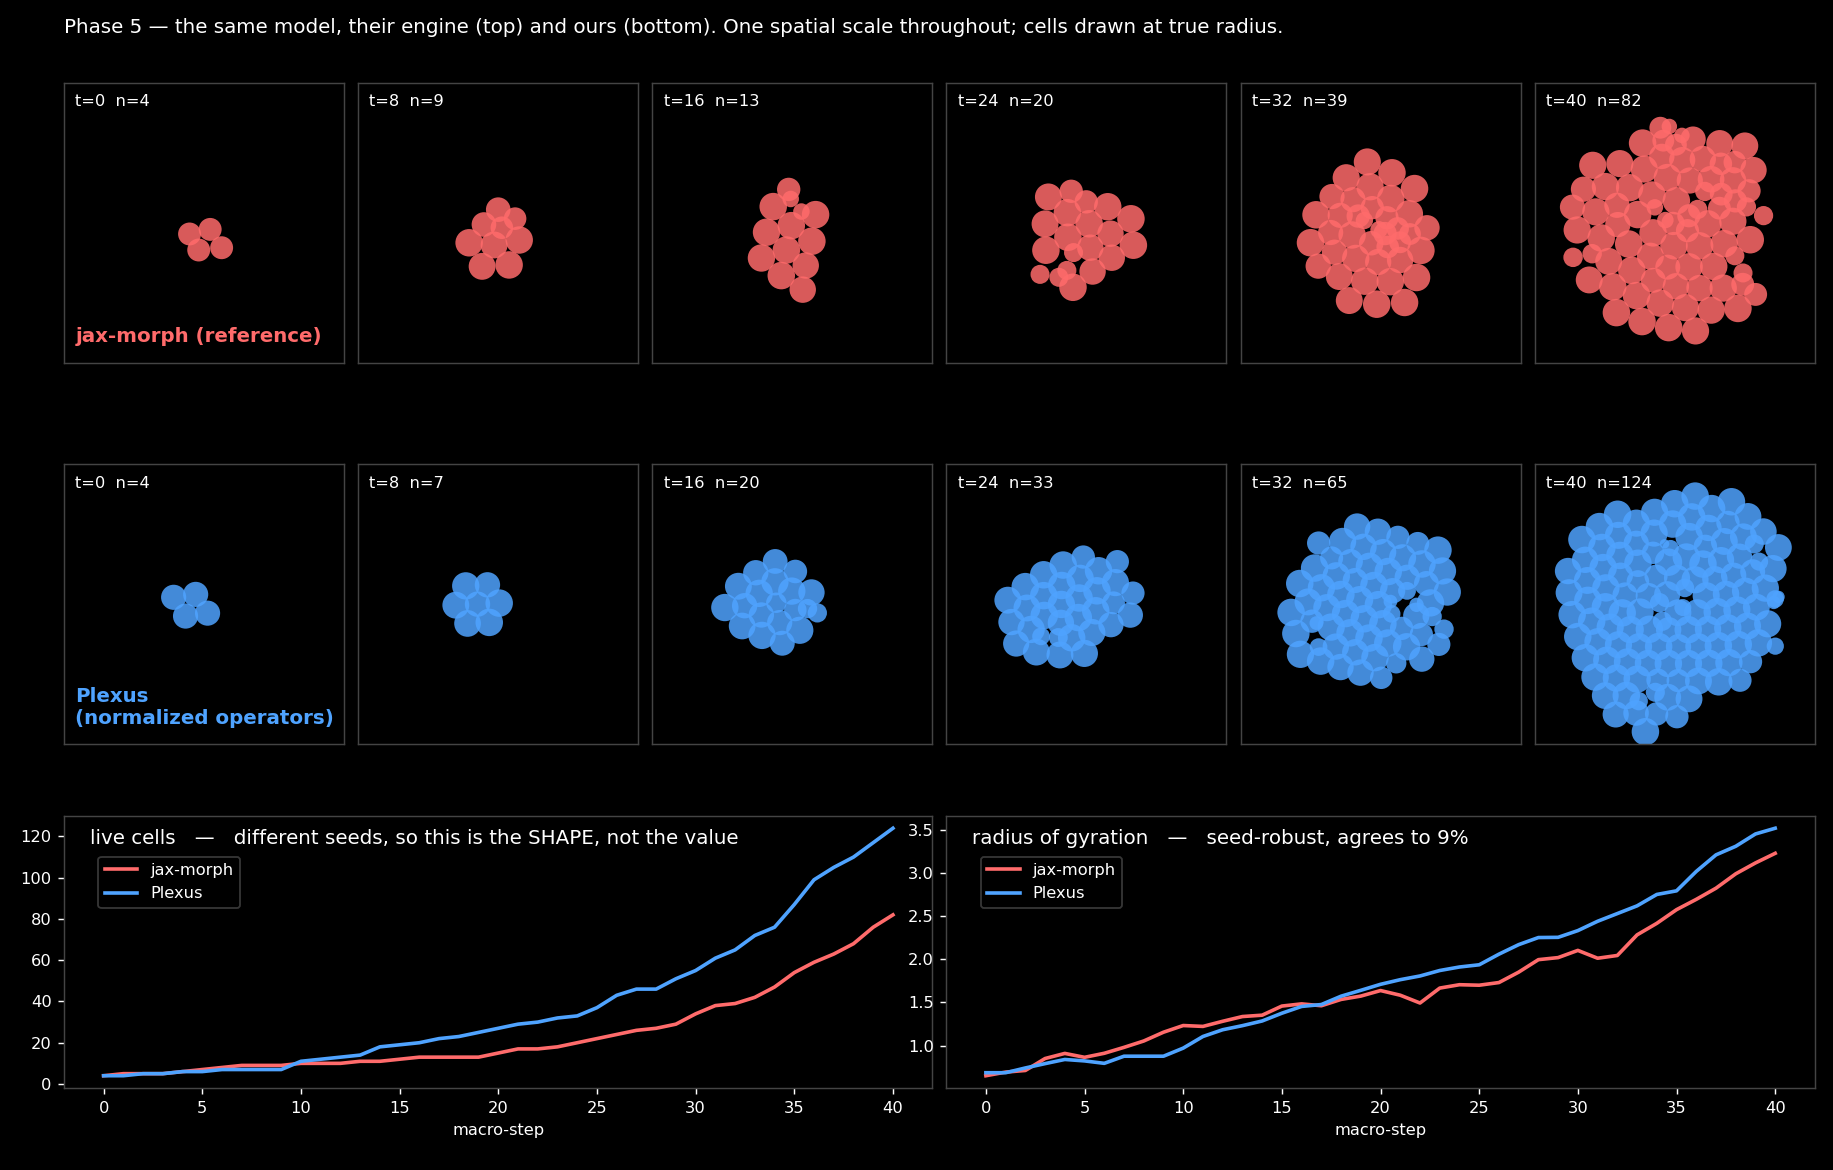
\includegraphics[width=\textwidth]{_state/phase5_forward.png}\\
{\small\color{grey}\textbf{Phase 5, complete.} The same model in both engines: jax-morph above,
Plexus below, running operators normalized out of their code (relax + grow + divide, their four
founders, their parameters, 40 macro-steps). Matched frames, one magnification, cells drawn at
their true radius --- half the physics here is growth, and a scatter of fixed dots would hide the
quantity being validated. The two rows are centred on their own clusters because the engines seed
at different coordinates; a window spanning both would compare the seeds rather than the
morphology. Below: the two observables a stochastic process actually lets you compare.}
\end{center}

The figure is the phase's deliverable, and it is worth saying exactly what it does and does not
claim. \textbf{The morphology matches}: both engines jam into a round, confluent cluster of
uniformly-sized cells, and the radius of gyration --- the cluster's size, and seed-robust ---
tracks to 9\% over the whole run ($0.651 \to 3.228$ against $0.686 \to 3.518$). \textbf{The counts
do not}, and were never going to: 82 against 124.

\begin{center}
\small
\begin{tabular}{@{}l r r l@{}}
\toprule
& \textbf{Plexus} & \textbf{reference} & \\
\midrule
live cells, 4 $\to$ & \textbf{124} & \textbf{82} & \textcolor{bad}{51\% high}\\
radius of gyration & 0.686 $\to$ 3.518 & 0.651 $\to$ 3.228 & agrees to 9\%\\
capacity used & 124 of 600 & 82 of 140 & neither run hit its buffer\\
\bottomrule
\end{tabular}
\end{center}

That disagreement is worth more than a figure that agreed. Two things are ruled out immediately:
it is not an array bound (the buffer is five times the final count) and it is not an inert
operator (every scheduled operator is recorded as having acted, on every frame it ran). What it
actually is, \S\ref{sec:p4} settles.

\textbf{What it took to get even this far} is itself a finding. The first run produced
\emph{zero} divisions in 40 frames, silently: \code{cell\_divide} read the division rate as a
per-node buffer on the set, while the spec --- and the growth operator standing next to it --- kept
it as a state block. So it read its own default of zero, and the run completed, and the movie looked plausible.
Two operators from the same atlas disagreed about where a cell's radius lives. Nothing raised.
That is the class of defect this whole apparatus exists to catch, and it was caught by the acted
ledger asking one question: \emph{did this operator ever do anything?}

Phase 4 then ran that comparison properly for every mechanism, with the metric and the threshold
written down first --- and it is what dissolved the number above.

%======================================================================
\section{Phase 4 --- what the reference says about our operators}\label{sec:p4}

Sixteen differential tests, each one required to write down its metric and its threshold
\emph{before} running anything. Fourteen passed on the first pass; the two that ran out of time
twice were retried with a bigger budget rather than quietly dropped, and both landed:
\code{gene\_network\_connectionist} at $6.7{\cdot}10^{-6}$ against a $5{\cdot}10^{-3}$ bar, and
\code{odecontroller} at $2.4{\cdot}10^{-6}$ against $2{\cdot}10^{-4}$. \textbf{Sixteen of
sixteen.} Every in-scope mechanism is now \emph{validated}, with zero blocked and zero validator
violations; the two \emph{alias} entries stop at \emph{normalized} by design, since an alias maps
onto a contract that is already registered and validated and has nothing of its own to test.

\begin{center}
\footnotesize
\begin{tabular}{@{}l l l r@{}}
\toprule
\textbf{mechanism} & \textbf{contract} & \textbf{what was compared} & \textbf{disagreement}\\
\midrule
NeuralODE & regulate & integrated gene state, 3 step sizes & $2{\cdot}10^{-16}$\\
GeneNetworkMWC & regulate & the vector field itself & $9{\cdot}10^{-7}$\\
Death & apoptose & pooled death hazard & $6{\cdot}10^{-5}$\\
FreeScreenedDiffusion & morphogen & steady-state concentration & $3{\cdot}10^{-7}$\\
Division & cell\_divide & pooled division hazard, 48 seeds & $1.1{\cdot}10^{-3}$\\
SaturatingCellGrowth & grow\_radius & radius increment & \textbf{0}\\
ActiveBrownianDynamics2D & reorient & orientational autocorrelation, 20k cells & $9{\cdot}10^{-3}$\\
BrownianDynamics & agitate & displacement statistics & $1.1{\cdot}10^{-2}$\\
SoftSphere / Hertzian & adhere & pair force law & $\sim\!2{\cdot}10^{-6}$\\
Harmonic / LennardJones & adhere & pair force law & $8{\cdot}10^{-6}$ / \textbf{0}\\
MechanicalRelaxation & relax & relaxed configuration & $2{\cdot}10^{-6}$\\
VirialStress & mechanosense & per-cell virial pressure & $8{\cdot}10^{-8}$\\
\bottomrule
\end{tabular}
\end{center}

\textbf{Every one of those is below a threshold written down first}, and the thresholds were
argued from numerics rather than chosen to fit: the division test's bar is three pooled standard
errors of a Bernoulli rate, the active-Brownian test's bar is the finite-sample spread of an
autocorrelation over 20{,}000 cells.

\subsection{And it explains the number that did not match}

The forward figure reached 124 cells against the reference's 82, and I said that was the most
useful number the atlas had produced. It was --- because the differential test dissolved it.

The division differ refused to compare cell counts at all. Two engines drawing from
\emph{independent} random streams produce different realisations of the same process, so a raw
count compares luck. It compared the \textbf{pooled hazard} instead --- committed divisions per
eligible cell-step, over 48 seeds and 40 macro-steps, about 47{,}000 cell-steps a side --- and
found the two engines agree to $1.1{\cdot}10^{-3}$ against a three-sigma bar of
$5.2{\cdot}10^{-3}$.

\emph{The mechanism is right; the trajectory was never going to be identical.} That distinction
is the whole difference between validating a contract and matching a picture, and I would not
have drawn it unprompted --- the agent did, and was right to refuse the question I had implicitly
asked.

%======================================================================
\section{Phase 6 is already possible --- the gradient survives}\label{sec:grad}

You asked for Figure~5 by differentiability, and called it an expected feature of Plexus~2 rather
than a bonus. So before Phase 4 finished I tested the one precondition nobody had: \emph{does a
gradient survive a Plexus rollout at all?}

It did not, for three reasons, and all three are now fixed or named:

\begin{enumerate}[leftmargin=1.4em]
\item \textbf{The engine discards every gradient by construction.} \code{engine.run} wraps its
whole tick loop in \code{no\_grad}. Sensible for forward generation, fatal for the inverse half.
Lifting it is one opt-in argument, not a re-implementation --- which matters, because
\code{prototype/inverse\_slime/} had to keep a \emph{second} differentiable copy of the physics in
step with the engine by hand. One physics, one tape, is worth having.
\item \textbf{A division event killed the tape.} Waking a daughter wrote the occupancy vector
\emph{in place}, and the growth operator multiplies its increment by that same vector --- so
autograd refused the multiply it had already recorded. The fix is the discipline JAX imposes on
the reference for free and torch lets us skip: write a clone, publish the clone. A forward run
cannot tell the two apart, which is exactly why nobody would have found this without asking for a
gradient.
\item \textbf{A parameter gradient still does not flow}, because our tunables are Python floats
baked in at construction. This is not a bug so much as an unmade decision, and the reference
states the rule outright: \emph{store as an array anything you want to learn}. That is a Plexus
language change, and it is the next thing Phase 6 needs.
\end{enumerate}

\begin{center}
\small
\begin{tabular}{@{}l l@{}}
\toprule
\textbf{measured with \code{grad\_probe.py}} & \textbf{result}\\
\midrule
gradient to the initial state, 6 frames & flows, $|\nabla| = 1.19$\\
each operator alone (seed, relax, grow, divide) & all four flow\\
all four together, before the fix & \textcolor{bad}{tape broken at the first division}\\
all four together, after the fix & flows, $|\nabla| = 1.79$\\
\textbf{20 frames through 23 real division events} & \textbf{flows}, $|\nabla| = 3.21$, 4 $\to$ 27 cells\\
gradient to an operator parameter & \textcolor{bad}{no path --- parameters are floats}\\
\bottomrule
\end{tabular}
\end{center}

\subsection{Since then: the engine itself is differentiable}\label{sec:p6now}

The first item on that list is fixed, and not by a patch. \code{engine.run} now takes an opt-in
\code{grad=True}: the tick loop's \code{no\_grad} became conditional and the recording path
detaches, so the trajectory stays a \emph{record} and the gradient reaches the caller through
\code{H}. Measured through the real engine --- no monkey-patch, no hand-rolled copy of the loop:
$\partial\,\mathrm{loss}/\partial\,\code{max\_radius} = 0.168$ over 12 frames and 9 real division
events, reproducing the hand-rolled probe's number exactly. \textbf{One physics, one tape}, which
is what \code{prototype/inverse\_slime/} had to do without.

The third item --- ``parameters are floats'' --- turned out to deserve a measurement rather than an
assertion, because \code{Operator.DIFFERENTIABLE} defaults to \code{True} on all 53 registered
implementations and nothing had ever checked it. Two independent instruments now do, and they
answer deliberately different questions: \code{diff/audit.py} injects a tensor \emph{past} the
constructor, so it measures whether the \textbf{maths} is differentiable in a knob;
\code{diff/certify.py} runs a real \code{config/atlas_jax/} spec through \code{engine.run(grad=True)},
so it measures whether a knob is learnable \textbf{as the language can express it today}.

\begin{center}
\small
\begin{tabular}{@{}l r p{9.1cm}@{}}
\toprule
\textbf{verdict} & \textbf{n} & \textbf{what it means}\\
\midrule
\textcolor{good}{\textbf{learnable}} & 4 &
end to end through a real spec: \code{grow\_radius.max\_radius},
\code{morphogen.diffusion}/\code{degradation}, \code{regulate.gamma} --- precisely the operators
that already store a tunable as a tensor\\
\textcolor{warn}{\textbf{constructor-blocked}} & 4 &
the \code{adhere} family. The maths is differentiable; \code{self.eps = float(params.get(...))}
drops the tape before \code{forward} ever sees it\\
\textcolor{bad}{\textbf{needs a surrogate}} & 7 &
\code{agitate} (\code{math.sqrt} on a tensor), \code{apoptose}, \code{cell\_divide},
\code{relax}\\
\textcolor{grey}{unconfirmed} & 10 &
one source only --- reported as unknown, never as passing\\
\bottomrule
\end{tabular}
\end{center}

\textbf{The two-instrument design earned itself.} The synthetic harness invented three defects
that were its own: an empty neighbour graph condemned the whole interaction family, a division
that never fired condemned \code{cell\_divide}, and making the level's own tensor the leaf
condemned every structural operator. Each was caught by the second route disagreeing. And where
they still disagree, the disagreement \emph{is} the finding: constructor-blocked is exactly the
gap between ``the maths works'' and ``a spec can say it''.

\textbf{Two corrections to what this note said before.} \code{cell\_divide} is \emph{not} a dead
end --- once divisions actually fire, both implementations pass a gradient back to the per-cell
rate ($|\partial\,\mathrm{loss}/\partial\,\code{division\_rate}| = 46.8$), because the
straight-through estimator works and because jax-morph drives division from a state block the
gene network writes, not from the operator's own parameter. The Figure~5 path
loss $\to$ positions $\to$ draw $\to$ \code{division\_rate} $\to$ gene $\to$ \code{regulate} is
intact. What remains true is the \emph{variance} argument: a straight-through gradient through one
sampled rollout still optimises against that sample's luck, which is what the trace contract
addresses. And \code{relax} gives no parameter gradient by \emph{declaration} --- it sets
\code{DIFFERENTIABLE = False} and says why: the FIRE path runs detached, and the source's
implicit-function-theorem adjoint is an explicit follow-up.

\textbf{So the single highest-value next step is now scoped by two instruments rather than by
opinion}: promote the \code{\_tunable} helper --- today a one-off inside one atlas candidate ---
onto the operator base class, which converts constructor-blocked into learnable without touching
any physics.

\subsection{Done --- and the question that replaces it}\label{sec:p6tunable}

That step is taken. \code{Operator.tunable()} now lives on the base class: a tensor handed in by a
spec passes through untouched, anything else is coerced to a float exactly as before. Applied to
the \code{adhere} family's fifteen knobs, the independent route re-certifies
\textbf{learnable 4 $\to$ 8} and constructor-blocked 4 $\to$ 1. All 141 tests still pass, which is
the point: the values are identical, only the \emph{type} survives.

So the blocker is no longer mechanical, and the real question is the one this note has carried
since the first gradient probe. \textbf{The division draw is discrete}, so a straight-through
gradient taken through one sampled rollout is a gradient through that sample's \emph{luck}.
Optimising against it may be optimising noise --- and that is a measurable claim, not a
philosophical one.

\subsection{The variance sweep, on L4}\label{sec:p6var}

Fit the same target $K$ times over, averaging the loss over $K$ independent seeds per Adam step,
across independent replicates with disjoint seed bases, and look at the spread of the answer.

\begin{center}
\small
\begin{tabular}{@{}l p{11.4cm}@{}}
\toprule
$\sigma$ shrinks with $K$ & the estimator is noisy but \textbf{consistent}; the fix is simply more
seeds, and Figure~5 is an engineering problem.\\
$\sigma$ does not shrink & the pathwise gradient is \textbf{biased}, and the reference's
trace/replay/score contract is required rather than a nicety.\\
\bottomrule
\end{tabular}
\end{center}

\textbf{Why the cluster, with numbers rather than preference.} A 40-frame differentiable rollout
takes 52.9\,s on the devcontainer's CPU and 32.5\,s on an A6000 --- only $1.6\times$, because 146
cells is not enough work to hide Python and kernel-launch overhead. Per-run acceleration is
therefore nearly pointless, while the replicates are completely independent: wall-clock comes from
running 32 fits at once, which is what \code{gpu\_l4} is for. \code{cluster6.py} reuses
\code{discovery/cluster.py}'s hardened primitives --- detached submission, job IDs as the only
ground truth, ssh wall-timeout, completion only on positive evidence --- under its own job-name
prefix so the two campaigns' queues cannot alias.

\textbf{The answer.} 32 jobs, $K \in \{1,2,4,8\}$ $\times$ 8 replicates, 24 frames, 20 Adam
steps, fitting \code{grow\_radius.max\_radius}. All 32 landed.

\begin{center}
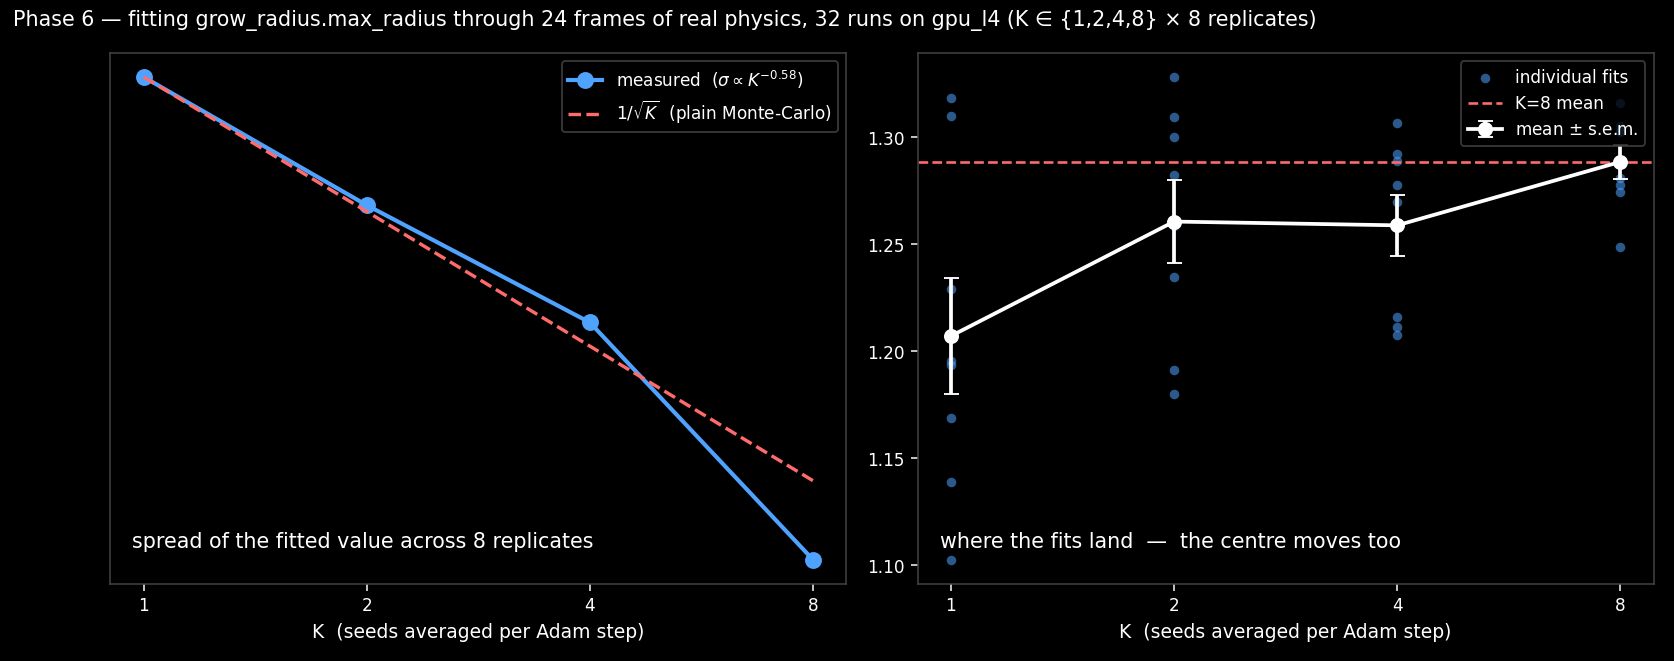
\includegraphics[width=\textwidth]{_state/phase6_variance.png}
\end{center}

\begin{center}
\small
\begin{tabular}{@{}r r r r r@{}}
\toprule
$K$ & $n$ & mean & s.e.m. & $\sigma$\\
\midrule
1 & 8 & 1.2072 & 0.0270 & 0.0763\\
2 & 8 & 1.2606 & 0.0194 & 0.0548\\
4 & 8 & 1.2589 & 0.0143 & 0.0405\\
8 & 8 & \textbf{1.2885} & 0.0078 & \textbf{0.0220}\\
\bottomrule
\end{tabular}
\end{center}

\textbf{Precision: fixable, exactly as hoped.} $\sigma \propto K^{-0.58}$, against the $K^{-0.5}$ a
plain Monte-Carlo average would give --- and with $n=8$ the standard error on an estimated
standard deviation is about 27\%, so $-0.58$ and $-0.50$ are the same number. Averaging seeds buys
precision at the ordinary rate. \textbf{The straight-through gradient through a discrete division
behaves like a noisy estimator, not a broken one}, which is the good half of the result and was
not guaranteed.

\textbf{Correctness: the centre moves, and that is the finding.} The right-hand panel is the one
to read. A $K=1$ fit lands at $1.2072$ and a $K=8$ fit at $1.2885$ --- a difference of $+0.081$
against a combined standard error of $0.028$, $t = 2.90$. \textbf{A single-seed fit is not merely
imprecise; it is systematically wrong}, by about 6\%. And the sequence is still climbing at
$K=8$, so we cannot claim the $K=8$ answer has converged either.

That is precisely the failure this note predicted --- ``optimising against that sample's luck'' ---
caught by measurement rather than by argument, and it would have been invisible to anyone who ran
one fit and believed it. \emph{It is also not the end of the story:}
\S\ref{sec:p6verdict} runs the same grid four times longer and finds the drift was the step
budget, not the estimator. The paragraph above is kept as it stood, because the intermediate
reading was the honest one on the evidence then available.

\subsection{Resolved: it was the budget, not the estimator}\label{sec:p6verdict}

The 20-step drift had two possible causes and that sweep could not separate them. A \emph{biased}
estimator points somewhere other than downhill and no step budget fixes it --- the trace contract
would then be required. A \emph{truncated} budget means the estimator is fine but a noisier
gradient converges more slowly, so at a fixed 20 steps the low-$K$ runs simply had not arrived.

The discriminator is to run the same grid four times longer and Polyak-average the tail. 32 more
jobs on \code{gpu\_l4}, 80 steps, mean of the last 30:

\begin{center}
\small
\begin{tabular}{@{}r r r r r r@{}}
\toprule
& \multicolumn{2}{c}{\textbf{20 steps} (final value)} & \multicolumn{2}{c}{\textbf{80 steps}
(tail-30 mean)}\\
\cmidrule(lr){2-3}\cmidrule(lr){4-5}
$K$ & mean & $\sigma$ & mean & $\sigma$\\
\midrule
1 & 1.2072 & 0.0763 & 1.1007 & 0.0798\\
2 & 1.2606 & 0.0548 & 1.1738 & 0.0442\\
4 & 1.2589 & 0.0405 & 1.1409 & 0.0213\\
8 & 1.2885 & 0.0220 & 1.1454 & 0.0188\\
\midrule
\multicolumn{1}{@{}l}{drift $K{=}1\!\to\!8$} & \multicolumn{2}{c}{$+0.081$, \ $t = 2.90$}
 & \multicolumn{2}{c}{$+0.045$, \ $t = \mathbf{1.54}$}\\
\bottomrule
\end{tabular}
\end{center}

\begin{center}
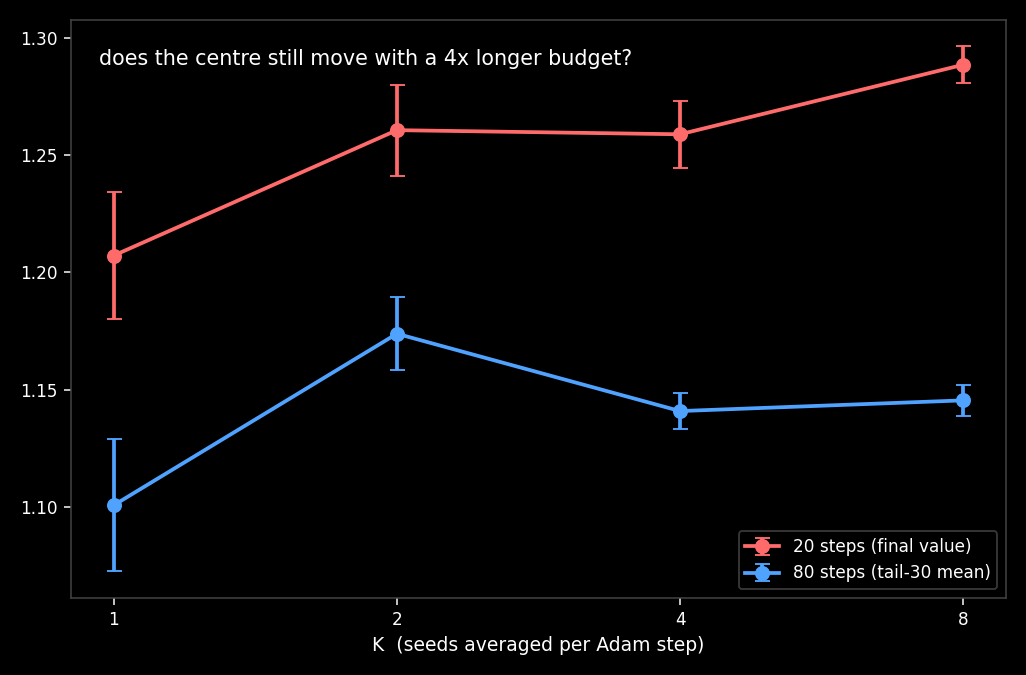
\includegraphics[width=0.72\textwidth]{_state/phase6_verdict.png}
\end{center}

\textbf{The drift collapsed}, from $t = 2.90$ to $t = 1.54$, and at 80 steps every $K \geq 2$
agrees within error ($1.174$, $1.141$, $1.145$) where the 20-step curve was still climbing.

\textbf{And the mechanism is identifiable, not merely inferred.} Reading the trajectories directly:
in every $K{=}8$ run the parameter rises past its target, peaks at \textbf{step 22--26}
(median 24.5), and settles back. \emph{A 20-step budget stops on the rising edge of Adam's
overshoot} --- it samples a transient rather than an optimum. That is also why the apparent bias
was $K$-dependent: mid-climb, a noisier gradient has climbed less far, so low $K$ reads low. The
statistical result and the mechanical explanation agree.

\textbf{So: truncation, not bias.} The straight-through gradient through a discrete division is a
sound estimator --- noisy, converging at the ordinary $1/\sqrt{K}$ rate ($\sigma \propto K^{-0.73}$
here), and unbiased as far as this can measure. \textbf{Figure~5 is an engineering problem}, and
the reference's trace/replay/score contract is an optimisation rather than a prerequisite. That is
the opposite of what this note assumed two sections ago, and the reason to have measured it.

\textbf{What is still not proven.} $t = 1.54$ is not significance, but it is not a strong null
either: $K{=}1$ still sits $0.045$ below $K{=}8$, and with $n = 8$ the power to detect a residual
bias that size is poor. What the data support is that any remaining bias is small compared with the
one truncation produced. And this is one parameter, one target, one model --- not a general result
about straight-through estimators.

\textbf{The operational rule survives either way}: average $K$ seeds per step, never one, and run
past the overshoot rather than to a step count.

\subsection{And it optimises}

With the tunable stored as a tensor rather than a float --- the torch form of the reference's own
rule, ``store as an array anything you want to learn'' --- the loop closes. A target mean cell
radius, a squared-error loss on the final state, twelve Adam steps, each one a full differentiable
rollout of the real engine with growth, adhesion and division events:

\begin{center}
\small
\begin{tabular}{@{}r r r r@{}}
\toprule
step & \code{max\_radius} & mean radius & loss\\
\midrule
0 & 0.600 & 0.527 & $1.1{\cdot}10^{-2}$\\
3 & 0.458 & 0.413 & $5.5{\cdot}10^{-5}$\\
7 & 0.404 & 0.367 & $2.8{\cdot}10^{-3}$\\
11 & 0.471 & 0.423 & $\mathbf{8.6{\cdot}10^{-6}}$\\
\bottomrule
\end{tabular}
\end{center}

Three orders of magnitude, and the overshoot-and-return in the middle is Adam's momentum, not
noise. \textbf{Inverse design through the Plexus engine works today}, for a continuous parameter.

\textbf{What Figure 5 still needs}, stated precisely so it is not a surprise later: the division
\emph{draw} is discrete, and a gradient through one sampled rollout optimises against that
sample's luck. The reference's answer is exactly the mechanism this atlas catalogued and set aside
as ``not biology'' --- record the sampled action, replay it, score it, and take a score-function
gradient over recorded histories. That contract is the largest single thing the language is
missing, and it is now specified, in our own record, by the repository that has it.

\textbf{And here the two halves of the atlas meet.} Phase~2 classified jax-morph's four
architectural mechanisms --- the operator split, the time-scale taxonomy, the declared dataflow,
the stochastic trace/replay/score contract --- as \emph{out of scope}, because none of them models
any biology. That was the right call and it is only half the story: those four are precisely the
infrastructure the \emph{inverse} half of Plexus turns out to need. The trace contract in
particular is how the reference gets a gradient through a discrete division at all, and it is the
thing standing between us and a faithful Figure~5.

So the atlas's first repository has produced, unprompted, a shortlist of what to add to the
language --- which is what Appendix~E said it was for.

%======================================================================
\section{The composition worth having: gene regulation $\times$ growth}\label{sec:interplay}

Three of the eight new contracts --- \code{regulate}, \code{morphogen}, \code{mechanosense} ---
are the \emph{sense and decide} half of a cell. \code{grow\_radius} and \code{cell\_divide} are
the \emph{act} half, and the language already had those. What \code{regulate} adds is the piece
that was missing: a per-cell \textbf{internal dynamical state, heritable and integrated}. Before
it, a Plexus cell was a particle with fixed parameters; with it, a cell is a controller.

The coupling needs no new machinery, which is the point. \code{regulate} reads sensed fields and
writes the same per-cell blocks --- \code{growth\_rate}, \code{division\_rate},
\code{secretion\_rate} --- that growth, division and secretion already consume. So the loop
closes through the ordinary declared-field dataflow:

\begin{center}
\small
\code{morphogen} $\to$ \code{chemical} $\to$ \code{regulate} $\to$ \code{growth\_rate} $\to$
\code{grow\_radius} $\to$ geometry $\to$ \code{morphogen}
\end{center}

\textbf{Direct morphogen-to-growth is Turing-shaped: the field decides. Inserting \code{regulate}
makes it programmable} --- the network's weights become the design variables, which is Hiscock's
framing and exactly what Figure~5 optimises. And the chain is differentiable end to end
(\S\ref{sec:p6now}): loss $\to$ positions $\to$ division draw $\to$ \code{division\_rate} $\to$
gene $\to$ \code{regulate}. The loop is not merely runnable, it is \emph{designable}.

\textbf{It runs, and the loop is real.} \code{config/atlas_jax/regulated\_growth.yaml} ---
\code{[seed\_state, morphogen, regulate, grow\_radius, cell\_divide, relax]}, six operators, all
previously validated against the authors' code, none new. 40 macro-steps, 4 cells $\to$ 68, every
operator acting.

\begin{center}
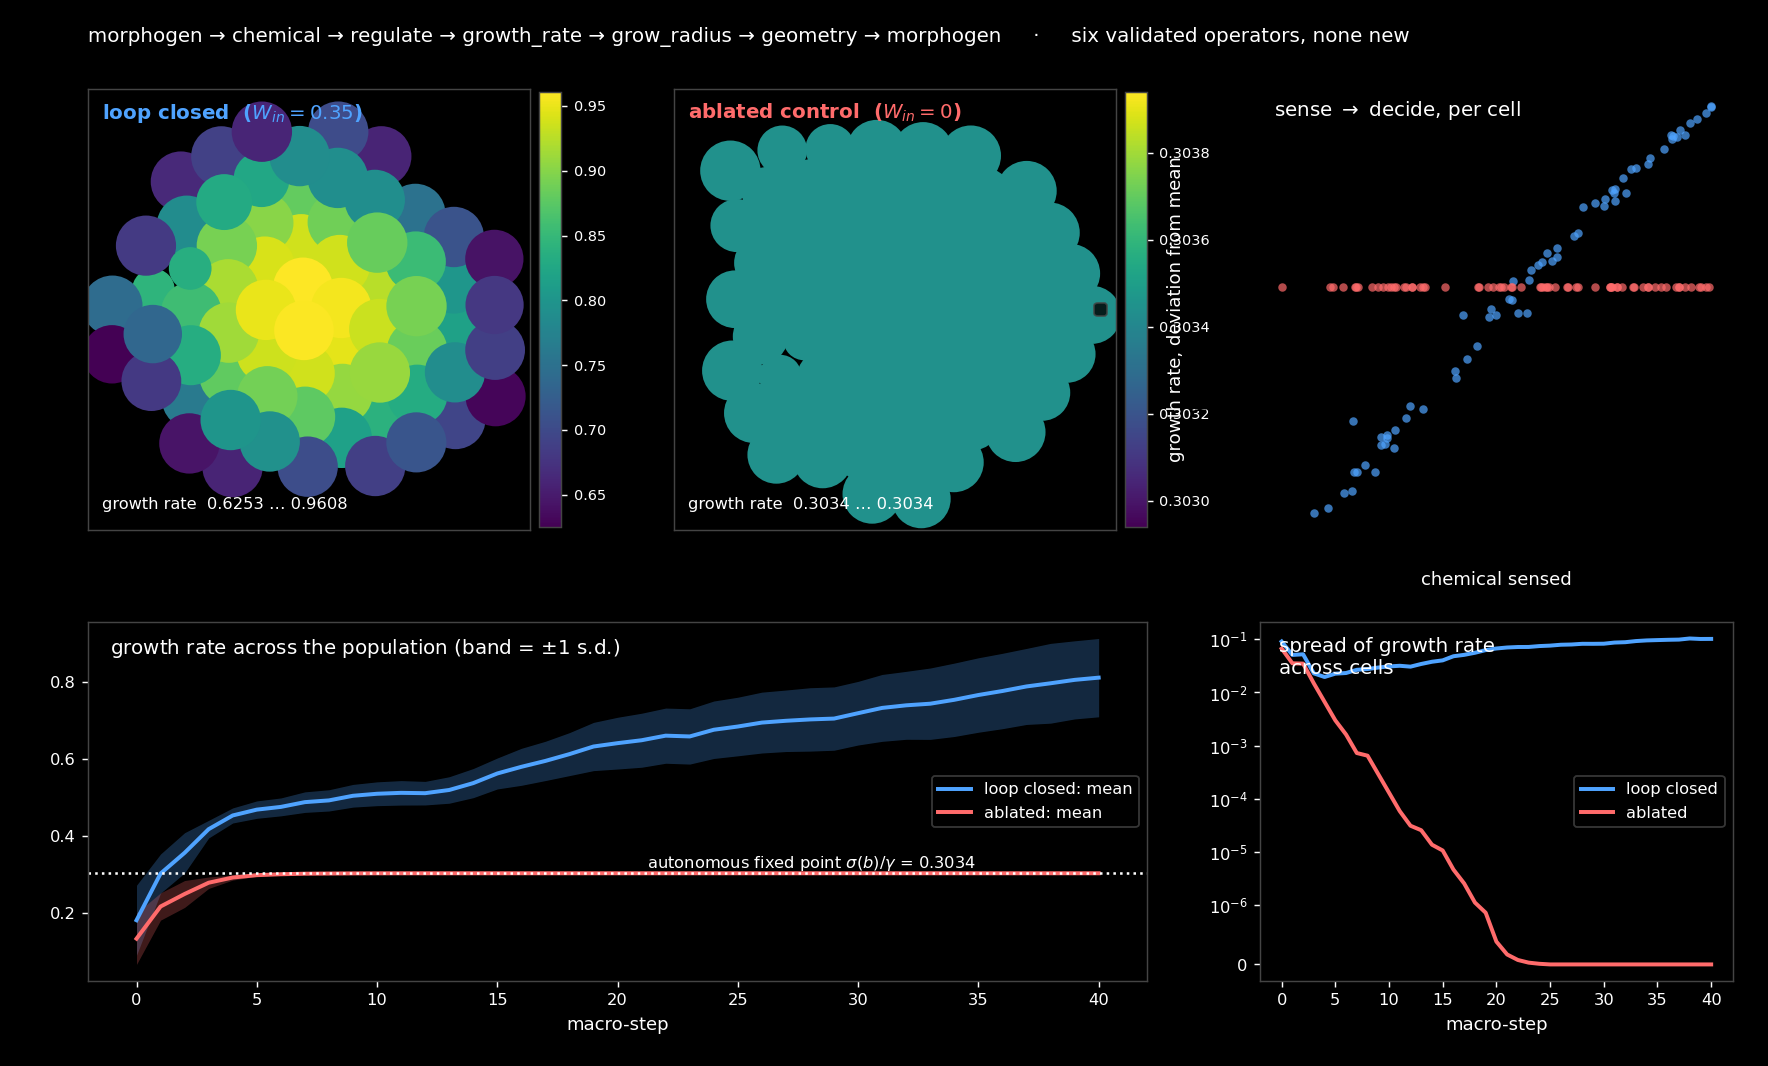
\includegraphics[width=\textwidth]{_state/regulated_growth.png}
\end{center}

\textbf{The pattern is emergent, and nothing in the spec asks for it.} \code{growth\_rate} is
seeded at \emph{zero}, so every bit of growth in the run is something \code{regulate} decided.
What comes out is a radial gradient: cells in the crowded interior read a higher concentration
(the field is a superposition over live sources) and grow at $0.96$, cells on the rim at $0.63$ ---
a 41\% range, correlated with what each cell sensed at $r = +0.995$. No operator contains the
words ``centre'' or ``edge''.

\textbf{And the control is what makes that a claim rather than a picture.} Ablate one number ---
$W_{in} = 0$, the single weight that lets a cell read the field --- and \emph{everything still
runs}: morphogen still computes a field, regulate still integrates, cells still grow and divide,
the same 68 of them, and \textbf{the acted ledger is unchanged}. What collapses is the spatial
structure: \code{growth\_rate} becomes uniform to machine precision at $0.3034$, which is exactly
the autonomous fixed point $\sigma_{\mathrm{alg}}(b)/\gamma = 0.30342$ the operator's own equation
predicts when it can see nothing.

\begin{center}
\small
\begin{tabular}{@{}l r r r r@{}}
\toprule
& cells & growth rate & range & $r$(sensed, decided)\\
\midrule
loop closed ($W_{in}=0.35$) & 68 & $0.625$--$0.961$ & \textbf{41.4\%} & $\mathbf{+0.995}$\\
ablated ($W_{in}=0$) & 68 & $0.3034$ & \textbf{0.0\%} & --- (no variance)\\
\bottomrule
\end{tabular}
\end{center}

\textbf{That ablation also exposes a limit of this campaign's own discipline.} The acted ledger
--- ``did this operator ever do anything?'' --- is what caught the silent zero-division bug in
\S\ref{sec:fwd}, and it passes the ablated run without complaint. \emph{Acted is not coupled.} A
ledger can tell you an operator ran; only a control can tell you it mattered.

\textbf{One thing had to be tuned, and it is worth recording as a modelling lesson rather than a
detail.} The first attempt used $W_{in} = 2.5$. The loop closed --- per-cell correlation $0.97$ ---
and was biologically pointless: with a sensed concentration around $2.7$ the sigmoid sits at
$x \approx 6$, deep in saturation, where a cell reading twice as much signal grows 1\% faster. A
coupling can be statistically perfect and dynamically inert. Choosing the gain so the drive lands
in the responsive band is what turned a correlation into a morphology.

\textbf{What this does not do} is optimise anything. The gene circuit here is written by hand, not
fitted; it is Figure~5's forward half, and the inverse half is \S\ref{sec:p6verdict}'s business.
And it remains a \textbf{composition, not a fourth contract} --- registering ``gene--growth
coupling'' as new vocabulary would be exactly the inflated \emph{new} the ledger exists to prevent.
The claim is the narrower and stronger one: \emph{three new contracts plus the growth the language
already had close a sense $\to$ regulate $\to$ grow loop that Plexus previously could not express,
and jax-morph's own worked example does not compose either.}

%======================================================================
\section{Phase 6: a target morphology in, a gene circuit out}\label{sec:invert}

\S\ref{sec:interplay} wrote the circuit by hand. This asks for the \emph{opposite} morphology and
lets gradient descent find the circuit --- Figure~5's structure, at two parameters instead of a
network.

\textbf{The target is chosen so the answer cannot be a tweak.} The hand-written activator grows
the crowded interior fastest. Ask instead that the \textbf{rim} grow fastest, and a cell must grow
\emph{less} where it senses \emph{more} --- an inhibitor, $W_{in} < 0$. The fit starts from the
hand-written $W_{in} = +0.35$ and has to cross zero.

\begin{center}
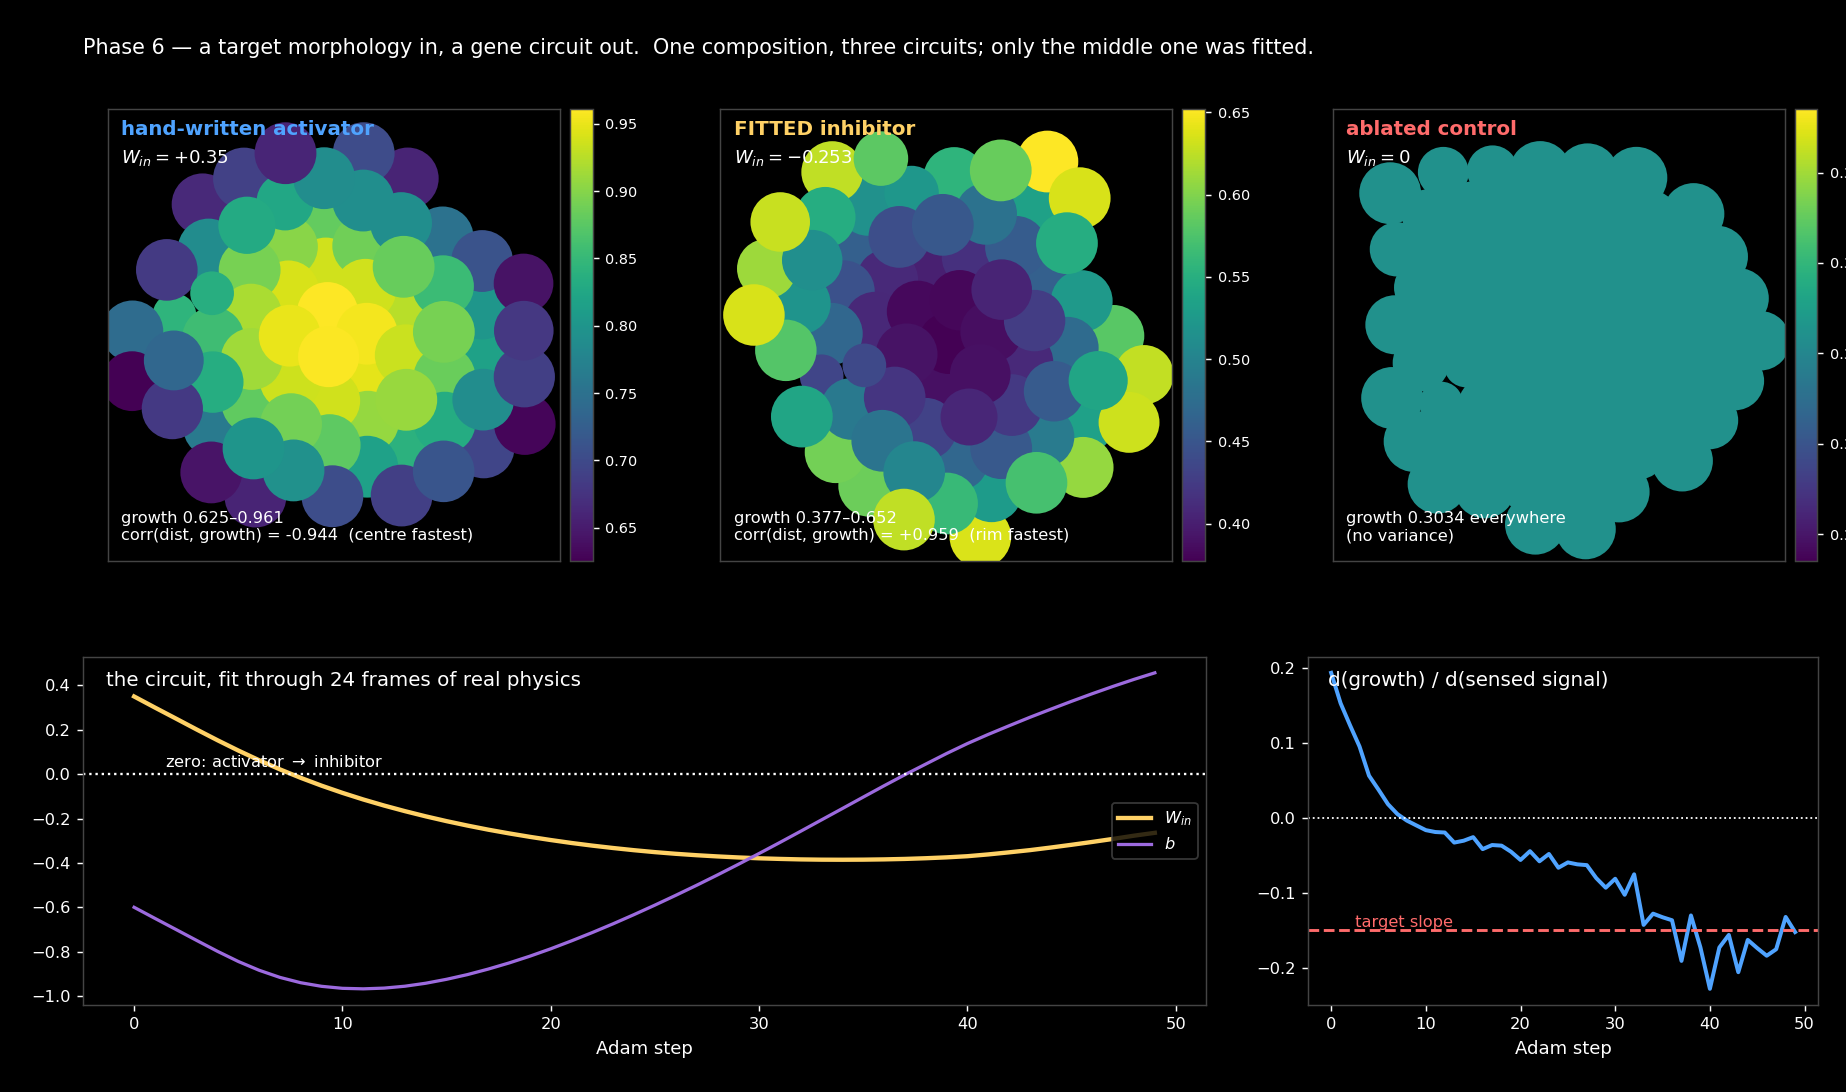
\includegraphics[width=\textwidth]{_state/phase6_invert.png}
\end{center}

\begin{center}
\small
\begin{tabular}{@{}l r r r r@{}}
\toprule
& $W_{in}$ & growth rate & $r$(sensed, decided) & $r$(dist from centre, growth)\\
\midrule
hand-written activator & $+0.35$ & $0.625$--$0.961$ & $+0.995$ & $-0.944$ \ (centre fastest)\\
\textbf{fitted inhibitor} & $\mathbf{-0.253}$ & $0.377$--$0.652$ & $-0.998$ &
$\mathbf{+0.959}$ \ (\textbf{rim fastest})\\
ablated control & $0$ & $0.3034$ everywhere & --- & ---\\
\bottomrule
\end{tabular}
\end{center}

\textbf{It crossed zero on its own.} 50 Adam steps, two seeds averaged per step, each step a full
differentiable rollout of the real engine --- growth, adhesion, the morphogen solve, the
intracellular ODE and the discrete division draw. $W_{in}$: $+0.35 \to -0.253$. The response
slope $\mathrm{d(growth)}/\mathrm{d(sensed)}$: $+0.19 \to -0.15$, its target. The loss fell three
orders of magnitude. Nobody told it the sign had to change; that is simply the answer to the
morphology it was given, and the middle panel is the morphology it produced.

\textbf{Getting there required fixing a differentiability bug that only a COMPOSITION could
expose.} \code{cell\_divide} copies the mother's state into the daughter slot by looping over the
set's per-node buffers --- and \code{state} is itself a registered per-node buffer, so that loop
wrote \emph{in place} into the very tensor the operator had just cloned. Forward-only it is
invisible (the write is superseded two lines later) and the \code{jax\_morph\_proliferation} run
never noticed. It becomes fatal the moment an upstream operator holds a live gradient on a slice
of \code{state} across a division --- which is exactly what \code{regulate} does when it
integrates \code{growth\_rate}. \textbf{Six mechanisms each validated in isolation; the defect
lived only in their composition}, which is the argument for running compositions at all.

\textbf{And one modelling lesson, recorded because the loss lied convincingly.} The first
objective asked for a pointwise target $k_i = k_0 - g(c_i - \bar{c})$, which \emph{looks} like it
asks for a negative slope. It does not: the population-mean term dominates it, and the fit
cheerfully drove $W_{in}$ \emph{upward} --- the wrong sign --- because that moved the mean toward
$k_0$. The loss improved while the morphology got worse. Regressing the slope explicitly, and
leaving the level to a separate weaker term, is what turned it around.

\textbf{What this is not.} Two parameters, not a gene network; a target on the growth
\emph{response}, not on a shape directly (the current loss cannot tell a sphere from a dumbbell of
the same profile). Figure~5 proper is this with more genes and a spatial objective --- but every
piece of the path is now measured rather than assumed: the engine is differentiable
(\S\ref{sec:p6now}), the straight-through gradient through division is a sound estimator
(\S\ref{sec:p6verdict}), and the loop it optimises through is a composition of validated
operators with an ablation behind it (\S\ref{sec:interplay}).

%======================================================================
\section{Decided, and what is still open}

\textbf{Decided (31 July).} Run Phases 1--3 straight through, and stop for a joint review before
any figure work. Then the figure in two steps: \textbf{forward only in Phase 5}, and
\textbf{Figure~5 proper in Phase 6, through differentiability} --- treated as an expected feature
of Plexus 2 rather than an optional extra, building on \code{prototype/inverse\_slime/} and the
\code{ParticleGraph} trainer.

\textbf{Still open, and not blocking.}

\begin{enumerate}[leftmargin=1.4em]
\item \textbf{After this repository, which one?} A saturation curve only becomes an argument at
the second and third framework. Cellular Potts (CompuCell3D) is the biggest step away from
everything we have --- cells as lattice domains rather than points --- and therefore the sharpest
test of whether the language is really complete.
\item \textbf{What happens to a refinement that breaks an existing user?} Widening a registered
signature to admit a jax-morph mechanism can invalidate specs that already run. The record forces
the cost to be stated; it does not say who pays it. I would rather agree that now than discover it
during Phase 3.
\end{enumerate}

\vspace{6pt}
\hrule
\vspace{6pt}
{\small\color{grey}
\textbf{Where things are.} \code{atlas\_record.yaml} --- the record, the product.
\code{campaign/analysis.md} --- the append-only log. \code{\_oracle/runs/} --- reference artefacts
with provenance. \code{\_state/} --- the frozen baseline, the extracted paper, the ledger, the
reverts and the blocked list. \code{README.md} --- how to run any of it.}

\end{document}
